
\section{Ecuaciones}
\subsection{Ecuaciones}\label{Ecuaciones}
Una ecuación es una igualdad entre dos expresiones que contienen una o mas
variables.  Esta es una expresión algebraica conformada una o mas variables y
operadores numéricos; estos se relacionan mediante operaciones como
suma, resta, multiplicación, división, potenciación, entre otras; y el objetivo
es conseguir el valor, o valores, de las variables que satisfacen la igualdad.
Una ecuación tiene la forma:
$$ \colorbox{RojoClaro}{13$x$ - 9}= \colorbox{AzulClaro}{5 + $x$} $$

Donde cada color representa un miembro de la ecuación, $x$ es la variable y se
puede observar que en cada miembro hay operaciones  suma, resta, y multiplicación


Para resolver una ecuación se procede a \comillas{despejar} la variable, este
proceso consiste
en agrupar todas las variables de un lado y todos los números del otro, realizar
las operaciones necesarias para simplificar y que de esta forma quede una única
variable igualada a un numero o una expresión. (por expresión se refiere a algún
tipo de función, como el valor absoluto, una raíz o una dependencia de otra variable
de forma que el resultado sea mas que un único dígito). Para resolver ecuaciones
se puede seguir la formula, algoritmo:


\begin{itemize}
    \item Colocar variables de un lado y los  números del otro. Esto se hace
        siguiendo ciertas \textbf{reglas}:
        \begin{itemize}
            \item Las \textbf{sumas} pasan como \textbf{restas}.
            \item Las \textbf{restas} pasan como \textbf{sumas}.
            \item Las \textbf{multiplicaciones} pasan como \textbf{divisiones}.
                \textbf{PERO}, tienen que estarse multiplicando a todo ese lado
                de la igualdad.
            \item Las \textbf{divisiones} pasan como \textbf{multiplicaciones}.
                \textbf{PERO}, tienen que estar dividiendo a todos los elementos
                de ese lado de la igualdad
            \item Los \textbf{exponentes} como raíces.\textbf{PERO}, tienen que
                estar abarcando a todos los elementos
                de ese lado de la igualdad
            \item Las \textbf{raíces} como exponentes. \textbf{PERO}, tienen que
                estar abarcando a todos los elementos
                de ese lado de la igualdad
        \end{itemize}
        Es decir se convierte en su \textbf{función inversa}.

    \item realizar las operaciones necesarias a ambos lados, son independientes,
        para simplificar la ecuación. \textbf{Cabe resaltar: }que las operaciones
        deben de realizarse siguiendo las reglas del álgebra, esto significa:
        \begin{enumerate}
            \item Paréntesis
            \item Exponentes
            \item Multiplicación y división
            \item Suma
        \end{enumerate}

        y si las operaciones tienen la misma jerarquía, del mismo nivel-tipo, se
        resuelven de izquierda a derecha.
        \textbf{Recordemos: } que hay un tipo especial de operación dentro de los
        exponentes, este se llama \refname{producto-notable}, y ocurre cuando la
        variable esta entre paréntesis en una operación de \textbf{suma o resta}
        y el paréntesis esta elevado a un exponente. Si no recuerda como resolverlo
        vaya a \refname{producto-notable}.
    \item En este punto deben de quedar expresiones sencillas a ambos lados de
        la igualdad, si no es que solo quedan números y una variable. por lo tanto:

        \textbf{Si la variable esta sola}: La ecuación esta resuelta(si la variable
        esta sola pero negativa se invierten los signos de la igualdad).

        \textbf{Si la variable esta siendo multiplicada o dividida}: se despeja
        para dejarla sola, se resuelve la operación resultante y este seria el
        resultado final
\end{itemize}

    Ejemplos: Resolver las siguientes ecuaciones:

    \begin{align*}
        13x - 9 &=5 + x		\\
        13x -x &= 5 +9\\
        12x &= 14 \\
        x &= \frac{14}{12} \\
        x&= \frac{7}{6}
    \end{align*}

    \begin{align*}
        124 + 18x -40 &= (19+45x)\times2 		\\
        \frac{124+18x-40}{2}&= 19 + 45x\\
        \frac{124}{2} +\frac{18x}{2} - \frac{40}{2}  &= 19 +45x\\
        \frac{18x}{2} -45x &= 19-\frac{124}{2} +\frac{40}{2} \\
        9x -45x &= 19-62+20\\
        -36x &=-23\\
        x &= \frac{-23}{-36} \\
        x &=\frac{23}{36}
    \end{align*}

    \begin{align*}
        (25x + 48)^2 -10 &= 666 \\
        (25x + 48)^2  &= 666+10 \\
        25x +48 &= \sqrt{676}\\
        25x + 48 &= 26 \\
        25x &= 26-48\\
        x &=  \frac{-22}{25}\\
    \end{align*}

    \begin{align*}
        \frac{150x+40 -65}{-50x +89}  &= 9 		\\
        150x+40-65 &= 9\times(-50x+89)\\
        150x -25 &= 9\times(-50x) + 9\times 89\\
        150x -25 &= -450x + 801\\
        150x + 450x &= 801 + 25\\
        600x &= 826\\
        x&=\frac{826}{600} \\
        x &= \frac{413}{300}
    \end{align*}

    \textbf{Notesé que: }la forma de resolver las ecuaciones siempre es la misma,
    se despeja hasta conseguir que todas las variables estén de un lado y todos
    los números del otro y se realizan las operaciones.

    \textbf{Consejo: } cuando se tienen fracciones o denominadores de un polinomio
    siempre suele ser mas sencillo buscar colocar de forma lineal, para esto se
    suele usar M.C.M o operaciones cruzadas hasta tener un denominador común,
    luego ese denominador se despeja.


\subsubsection{Forma canónica de la ecuación}
    Este es un caso particular de las ecuaciones, y es de suma importancia para
    el estudio y la resolución de las mismas. Se dice que una ecuación esta en
    su \textbf{forma canónica} cuando uno de sus miembros, lados, es 0 y el otro
    miembro no puede ser simplificado mas, es decir
    hay una expresión igualada a 0.

    La importancia de este tipo de ecuaciones es que facilitan la resolución en
    ciertos casos y en otros permiten la interpretación de un fenómeno físico con
    mayor claridad. \textbf{Recordemos} que las matemáticas son utilizadas para
    describir el comportamiento y la evolución de fenómenos físicos para de esta
    forma entender a mayor profundidad el mundo que nos rodea.

    La forma de resolver una ecuación en forma canónica es la misma que la
    explicada anteriormente. y para colocar una ecuación a su forma canónica basta
    con pasar todos los elementos a un mismo lado,siguiendo las reglas del despeje.
    Ejemplos:

    Llevando las ecuaciones anteriores a su forma canónica:

    \begin{align*}
        13x - 9 &= 5 + x		\\
        13x -x -9 -5 &= 0\\
        12x -14 &= 0 \\
    \end{align*}

    \begin{align*}
        124 + 18x -40 &= (19+45x)\times2 		\\
        \frac{124+18x-40}{2}&= 19 + 45x\\
        \frac{124}{2} +\frac{18x}{2} - \frac{40}{2}  &= 19 +45x\\
        \frac{124}{2} +\frac{18x}{2} - \frac{40}{2} -19 -45x  &=0\\
        62+9x-20-19-45x=0
        -36x+23 &= 0\\
    \end{align*}

    \begin{align*}
        (25x + 48)^2 -10 &= 666 \\
        (25x + 48)^2  &= 666+10 \\
        25x +48 &= \sqrt{676}\\
        25x + 48 &= 26 \\
        25x +48 -26 &= 0 \\
        25x+22 &= 0\\
    \end{align*}

\subsubsection{Tipos de ecuaciones}
    Existen muchos tipos de ecuaciones, estas se clasifican por el tipo de operaciones
    que son necesarias para resolverlas. La clasificación mas común, y la que se
    estudiara es la de \textbf{ecuaciones algebraicas}, esta recibe este nombre
    dado que para resolverla solo hacen falta operaciones algebraicas.

    \textbf{Cabe resaltar} que existen otro tipo de ecuaciones como las logarítmicas
    diferenciales, integrales y funcionales, estas no se estudiaran ya que
    pertenecen a cursos mas avanzados.

    Las \textbf{ecuaciones algebraicas}, se suelen sub dividir según \textbf{el
    grado} del polinomio en:

    \begin{itemize}
        \item De primer grado o lineales.
        \item De segundo grado o cuadráticas.
        \item De tercer grado o cubicas.\\
        \vdots
        \item De grado n, n $\in\mathbb{N}$.
    \end{itemize}
    \textbf{recordemos} que el grado de un polinomio es
    \textbf{el exponente mas alto al que esta elevado la variable independiente}.

    \subsubsection*{Ecuaciones 1er orden} \label{Ecuaciones-1er-orden}
    Su forma canónica es: $ax+b=0;\ a,b\in\mathbb{R}$ $a$ es llamado coeficiente
    de $x$ y $b$ es el termino independiente.

    Este tipo de ecuaciones se resuelven de la forma previamente estudiada, es
    decir se despeja la x siguiendo las reglas anteriormente nombradas. Ejemplo:

    \begin{align*}
        10x +50 &= 3		\\
        10x &= 3-50 \\
        x &= \frac{-47}{10} \\
        x &= -4.7\\
    \end{align*}

   \begin{align*}
       (95x -10)^3 &= 27		\\
       95x -10 &= \sqrt[3]{27} \\
       95x &= 3 +10\\
       x &= \frac{13}{95} \\
   \end{align*}



    \subsubsection*{Ecuaciones 2do orden} \label{Ecuaciones-2do-orden}
    Su forma canónica es: $a_1x^2+a_2x+b=0;\ a,b\in\mathbb{R}$ $a_1,a_2$ son
    llamados coeficientes  de $x$ y $b$ es el termino independiente.

    Para resolver este tipo de ecuación se busca expresarlo en su forma canónica
    y aplicar una formula, a esta se le suele llamar \textbf{resolvente cuadrática},
    o solo \textbf{resolvente} pero al ser tan utilizada se le conoce de muchas
    formas\dots

    \textbf{Cabe resaltar que:}
    también se puede escribir la forma canónica de la forma:
    $ax^2+bx+c=0$, es lo mismo, pero la formula que se usa para resolver este tipo
    de ecuaciones suele llevar $a,b,c$.

    La formula a usar es:

    $$x = \frac{-b \pm \sqrt{b^2 - 4ac}}{2a} $$


    donde $a,b,c$ son respectivamente los coeficientes de la formula.

    También se observa que existe un símbolo $\pm$ este indica que pueden haber
    \textbf{2 resultados posibles que satisfacen la ecuación}. Para conseguirlos
    se tiene que resolver 2 veces todos los cálculos, \textbf{1 vez sumando} y
    \textbf{1 vez restando}, es decir, $\pm$ se va a reemplazar por un + para
    $x_1$ y por un - para $x_2$.    Ejemplos:



    \begin{align*}
        x^2 + 5x -14 &= 0		\\
        \text{identificamos que: }& a=1,b=5,c=-14\\
        \text{entonces, procedemos a }&\text{sustituir en la formula:}\\
        x &= \frac{-5\pm \sqrt{5^2-4\times1\times-14}}{2\times1}\\
        x &= \frac{-5\pm \sqrt{25+56}}{2}\\
        x &= \frac{-5\pm \sqrt{81}}{2}\\
    \end{align*}
        Luego, realizamos las 2 operaciones:
     \begin{align*}
         x_1 &= \frac{-5 +\sqrt{81}}{2} &  x_2 &= \frac{-5 -\sqrt{81}}{2}\\
         x_1 &= \frac{-5 +9}{2} & x_2 &= \frac{-5 -9}{2}\\
         x_1 &= \frac{4}{2} &  x_2 &= \frac{-14}{2}\\
         x_1 &= 2 &  x_2 &= -7
    \end{align*}

    Algunas veces la raíz interna no es exacta, en esos casos se deja expresado:
    \begin{align*}
        x^2 + 5x -9 &= 0		\\
        \text{identificamos que: }& a=1,b=5,c=-9\\
        \text{entonces, procedemos a }&\text{sustituir en la formula:}\\
        x &= \frac{-5\pm \sqrt{5^2-4\times1\times-9}}{2\times1}\\
        x &= \frac{-5\pm \sqrt{25+36}}{2}\\
        x &= \frac{-5\pm \sqrt{61}}{2}\\
        \text{y entonces, queda }&\text{de la forma:}\\
        x_1 = \frac{-5 +\sqrt{61}}{2}\ ;&\ \ \  x_2 = \frac{-5 -\sqrt{61}}{2}
    \end{align*}

    En otras ocasiones se tendrá que despejar antes de aplicar la formula:

    \begin{align*}
        4x +186 &= -10x + 5x^2 \\
        -5x^2 +4x+10x+186 &= 0\\
        -5x^2 +14x+186 &= 0\\
        \text{identificamos que: }& a=-5,b=14,c=186\\
        \text{entonces, procedemos a }&\text{sustituir en la formula:}\\
        x &= \frac{-14\pm \sqrt{14^2-4\times-5\times186}}{2\times-5}\\
        x &= \frac{-14 \pm \sqrt{196+3720}}{-10}\\
        x &= \frac{-14 \pm \sqrt{3916}}{-10} \\
        \text{y entonces, queda }&\text{de la forma:}\\
        x_1 = \frac{-14+\sqrt{3916}}{-10}\ ;&\ \ \  x_2 = \frac{-14 -\sqrt{3916}}{-10}
    \end{align*}

    Y en algunos casos la raíz se hará 0 y se terminara con que ambos valores
    serán el mismo:

    \begin{align*}
        x^2 +4x x_1=x_2&=-2+4 &= 0		\\
        \text{identificamos que: }& a=1,b=4,c=4\\
        \text{entonces, procedemos a }&\text{sustituir en la formula:}\\
        x &= \frac{-4\pm \sqrt{4^2-4\times1\times4}}{2\times1}\\
        x &= \frac{-4 \pm \sqrt{ 16 - 16}}{2} \\
        x &= \frac{-4\ \pm 0}{2}\\
        \text{ y por lo tanto }&\text{$x_1$ y $x_2$ valen: -2}\\
        x_1=&x_2=-2
    \end{align*}




    \subsubsection*{Ecuaciones de 3er orden o superior} \label{Ecuaciones-de-3er-orden-o-superior}
    Su forma canónica es: $a_1x^3+a_2x^2+a_3+b=0;\ a,b\in\mathbb{R}$ $a_1,a_2,a_3$ son
    llamados coeficientes  de $x$ y $b$ es el termino independiente.

    La forma general es:
    $$a_1x^n+a_2x^{n-1}+a_3x^{n-2}+\cdots+a_{n+1}x+b = 0$$
    donde, $a_1,a_2,a_3,\cdots,a_{n+1}$ son los coeficientes, $b$ es el termino
    independiente y todos estos son números reales. $n$ es llamado exponente máximo,
    representa el grado y puede ser cualquier numero natural ($n \in \mathbb{N}$)


    Este tipo de ecuaciones se resuelven al factorizarla, ya que de esta forma
    se consiguen las raíces. La forma mas común es utilizando el método
    de \textbf{Ruffini}. Véase (\refname{Factorización}) para una explicación
    mas profunda.
    Ejemplos:

    \textbf{Recordemos que:} las raíces son los valores que hacen 0 el polinomio-
    expresión y que por lo tanto hacen cumplir la igualdad en la forma canónica
    ($expresión=0$).

    Se pueden presentar varios casos, cuando no hay termino independiente:
    \begin{align*}
        x^3 + 5x^2 -14x &=0 		\\
        \text{Procedemos a factorizar} &\text{primero factor común }x \\
        x(x^2 + 5x -14)&=0\\
        \text{Luego, nos queda una ecuación }& \text{de segundo grado, ejemplo anterior:}\\
        \text{donde: }  x_1 = 2 &  x_2 = -7\\
        \text{por lo tanto la ecuación} & \text{factorizada resultante es:}\\
        x\times(x-2)\times(x+7)&= 0\\
        \text{y los resultados}& \text{de la ecuación son: } \\
        x_1= 2,\ x_2&=-7,\ x_3=0\\
    \end{align*}

    \textbf{Notemos:} que se busca factorizar la expresión, al sacar factor común
    buscamos que nos quede un termino independiente, en ese momento procedemos,
    según el grado del polinomio resultante, a usar la resolvente cuadrática o
    Ruffini.

    cuando hay termino independiente:
    \begin{align*}
        2x^3+9x^2+13x &= -6\\
        \text{despejando, }& \text{a su forma canónica:}   \\
        2x^3+9x^2+13x+6 &= 0\\
        \text{Como \textbf{HAY} termino independiente, no se }& \text{puede usar factor común} \\
        \text{procedemos por Ruffini:Los coeficientes, en}& \text{ orden decreciente, son: } 2,\ 9,\ 13,\ 6;
    \end{align*}

\begin{center}
     \begin{tabular}{c|cccc}
            &  2&  9&  13&  6\\
        -1  &   & -2&  -7& -6\\\hline
            &  2&  7&   6&  0\\
        -2  &   & -4&  -6\\\hline
            &  2&  3&   0\\
$\frac{-3}{2}$&   & -3&  \\\hline
            & 2 & 0
    \end{tabular}
\end{center}

    La ecuación factorizada, resultante seria:
    $$ (x+1)\times(x+2)\times\left(x+\frac{3}{2}\right)= 0  $$

    y por lo tanto, las soluciones serian: $x_1 = -1, x_2 = -2, x_3=\frac{-3}{2} $

\subsection{Inecuaciones}

    Una inecuación es una desigualdad algebraica, estas son un equivalente de las
    \refname{Ecuaciones} pero con los operadores relacionales $<,>,\leq,\geq$.
    Además, las inecuaciones dan como resultado un \textbf{conjunto de valores}
    los cuales cumplen la desigualdad, mientras que la ecuación daba un numero,
    mas si era de un grado mayor.

    Asimismo, las inecuaciones también obedecen a una regla la cual modifica el
    operador relacional entre los términos:

    \textbf{Si se multiplican o dividen ambos términos de una inecuación por un
    numero negativo, el operador relacional se invierte}. Esta inversión es como
    sigue:

    \begin{itemize}
        \item el < pasa a ser >.
        \item el > pasa a ser <.
        \item el $\leq$ pasa a ser $\geq$.
        \item el $\geq$ pasa a ser $\leq$.
    \end{itemize}

    Esto implica que: \textbf{si hay igualdad, esta se mantiene} ($\leq,\ \geq$).
    \textbf{Recuerde que:} cuando se pasa un numero a multiplicar o dividir al
    otro lado de la desigualdad, es
    el equivalente a multiplicar o dividir (respectivamente) ambos lados por ese
    numero. Entonces, \textbf{cuando se despeja un numero negativo que multiplica
    o divide se invierte el operador relacional}.

    \textbf{Es importante} resaltar que las inecuaciones pueden ser representadas
    de forma gráfica, ya que son un conjunto de puntos en la recta real. véase
    \refname{Grafica-inecuaciones}.


    Ejemplo y explicación:

    \begin{align*}
        5x + 40 & < 0\\
        5x  & < -40\\
        x & < \frac{-40}{5} \\
        x & < -8 \\
    \end{align*}

    Entonces, la solución es el conjunto de valores que puede tomar x que sean
    menores a -8, es decir \{ -9, -10, $\displaystyle\frac{-354}{2} $, -354,$\cdots$, $-\infty$   \}
    Es decir todos los numero $x \in \mathbb{R}$ (si se trabaja en otro conjunto
    $\{\mathbb{N},\mathbb{Z},\mathbb{Q}\} \text{se usa ese conjunto en vez de }\mathbb{R}$)
    que cumplen $\{x \in \mathbb{R}:x < -8\}$, otra forma: el conjunto $(-\infty;-8)$.

    Se pueden observar que, el proceso de despeje sigue siendo el mismo mas hay
    un paso adicional, \textbf{conseguir el conjunto solución}; este puede ser
    expresado de 2 formas, como: $\{x \in \mathbb{R}:x < -8\}$ o de la forma
    $(-\infty;-8)$. Ambos resultados son exactamente iguales, la segunda forma
    es la mas vista en bachillerato, sin embargo el primero suele
    ser usado en niveles mas avanzados ya que da mas libertad y permite definir
    expresiones mas complejas.

    Para expresar el resultado en forma de conjunto se debe hacer lo siguiente:

    \textbf{Es importante saber: }


\begin{table}[H] \label{operadores-relacionales-a-conjuntos}
    \begin{adjustwidth}{-.5in}{-.5in}
        \begin{center}

            \begin{tabular}{|c|c|c|}
                \hline


                Operador relacionar & Nombre                        & expresión como conjunto\\\hline
                <                   & Menor que o menor estricto    & " ) " = paréntesis de cierre \\\hline
                >                   & Mayor que o mayor estricto    & " ( " = paréntesis de apertura\\\hline
                $\leq$              & Menor o igual que             & " ] " = Bracket (corchete cuadrado) de cierre \\\hline
                $\geq$              & Mayor o igual que             & " [ " = Bracket (corchete cuadrado) de apertura \\

                \hline
            \end{tabular}

        \end{center}
    \end{adjustwidth}
\end{table}

    \subsubsection*{Primera forma}
    Primero, la forma de decirlo es: $\{x \in \mathbb{R}:x < -8\}$
    sea $x$ perteneciente($\in$) a los reales ($\mathbb{R}$) tal que(:)
    $x$ es menor que -8 (también se puede decir: menor estricto que -8).

    y para escribirlo solo hay que escribir:

    $$ \{ \text{variable} \in \text{conjunto} : \text{inecuación final}  \} $$

    En el caso del ejemplo anterior
   \begin{itemize}
        \item  variable: $x$
        \item conjunto no se especifico, así que asumiremos $\mathbb{R}$ ya que
            es el mas general, e
        \item expresión: $x<-8$
   \end{itemize}

    y al reemplazar obtenemos el resultado: $\{x \in \mathbb{R}:x < -8\}$

    \subsubsection*{Segunda forma} \label{Segunda-forma}
    La forma de decirlo es:  $(-\infty;-8)$ el conjunto formado por los números
    desde menos infinito hasta -8 abierto .

    Para escribirlo hay que tener en cuenta

    \begin{itemize}
        \item Cuantos factores-conjuntos tiene, esto es ya que como se vera mas adelante,
            cuando se tienen polinomios de un grado alto, en valor absoluto o en
            forma de fracción se crean mas de 1 conjunto solución.
        \item El tipo de desigualdad, de acuerdo a esto se reemplazara según la tabla
            \ref{operadores-relacionales-a-conjuntos}.
        \item \textbf{El infinito siempre va con corchete}, ya sea de apertura o de
            cierre, dependiendo de su ubicación.
    \end{itemize}

    Se toma en cuenta la forma de la desigualdad, se identifican los términos, cual
    es el mayor y cual es el menor y siguiendo las normas anteriormente
    nombradas se coloca:

    \begin{itemize}
        \item " ( " o " [ ", dependiendo del operador, y la consideración del infinito.
        \item expresión de menor valor en la desigualdad.
        \item ;
        \item expresión de mayor valor de la desigualdad.
        \item " ) " o "] ", dependiendo del operador, y la consideración del infinito.
    \end{itemize}

    De esta forma se tiene que:

    Menor valor = $-\infty$

    Mayor valor = -8

    Entonces: $(-\infty;-8)$

\subsubsection{Gráfica de inecuaciones} \label{Grafica-inecuaciones}

    Las inecuaciones pueden ser vistas de una forma gráfica, como un
    conjunto de puntos en la recta real. El punto de inicio suele ser un circulo
    o punto abierto, o paréntesis, para los intervalos abiertos, creados con "<" o ">"
    y un punto o circulo coloreado, o corchetes para los intervalos cerrados, los
    creados con $ \leq $ $ \geq $.

    Para crear la gráfica se debe:

    \begin{enumerate}
        \item Dibujar la \textbf{Recta real}. \textbf{Recordemos que:} esta es una
            linea en la cual se coloca un punto medio, 0, y a su derecha los números
            positivos y a su izquierda los números negativos, siguiendo el orden
            numérico tradicional ($\cdots,-2,-1,0,1,2,\cdots$).

        \item Marcar los puntos de especial importancia, estos son el 0, como
            referencia o valor, y luego todos \textbf{los puntos críticos.}

            Lo \textbf{puntos críticos} son los números en los cuales se hace 0
            una ecuación, para conseguirlos lo que se hace es reemplazar \textbf{
            EN LA ULTIMA EXPRESIÓN DE LA INECUACIÓN}, es decir cuando se tiene
            resuelto, y  conseguir los valores solución de esta, a veces es mas
            fácil expresarla en su forma canónica.

        \item Comprobar hacia que lado se cumple la desigualdad y marcarlo.

            Para esto es suficiente con tomar un punto de prueba a la derecha o
            izquierda del punto critico, o en un intervalo especifico, y comprobar
            si ese valor satisface la desigualdad, si es así, todos esos puntos
            forman parte del intervalo solución. Por lo tanto se marcan.:w

    \end{enumerate}

    Algunos ejemplos son:

    \textbf{Para: } $x>0$

    Recta:

    \vspace*{1cm}
    \begin{tikzpicture}[scale=3]
        %Eje y numeracion
        \begin{scope}
            \draw[->] (-1.5,0) -- (1.5,0)node[right] {$x$}coordinate(x axis);
            \draw (-1.5,0) node[below] {$-\infty$}coordinate(x axis);
            \draw (1.5,0) node[below] {$\infty$}coordinate(x axis);
            \foreach \x/\xtext in {-1, 0, 1/-1,0,1}
            \draw[xshift=\x cm] (0pt,1pt) -- (0pt,-1pt) node[below,fill=white] {$\xtext$};
        \end{scope}
    \end{tikzpicture}


    Puntos: 0 únicamente. infinitos de referencia.

    \vspace*{1cm}
    \begin{tikzpicture}[scale=3]
        %colores
        \colorlet{w}{green!20!white}
        \colorlet{bblue}{blue!60!black}

        %puntos
        \filldraw[red!50!white] (0,0) circle (0.8pt);

        %Eje y numeracion
        \begin{scope}
            \draw[->] (-1.5,0) -- (1.5,0)node[right] {$x$}coordinate(x axis);
            \draw (-1.5,0) node[below] {$-\infty$}coordinate(x axis);
            \draw (1.5,0) node[below] {$\infty$}coordinate(x axis);
            \foreach \x/\xtext in {-1, 0, 1/-1,0,1}
            \draw[xshift=\x cm] (0pt,1pt) -- (0pt,-1pt) node[below,fill=white] {$\xtext$};
        \end{scope}
    \end{tikzpicture}


    Comprobando con $x=1,\ 1>0 $? si, por ende se cumple y es hacia la derecha
    del \textbf{punto critico} 0.

    Marcas: dado que es una desigualdad abierta (<) el circulo va abierto o se
    usa un paréntesis

    Con paréntesis:

    % inmayor
    \vspace*{1cm}
    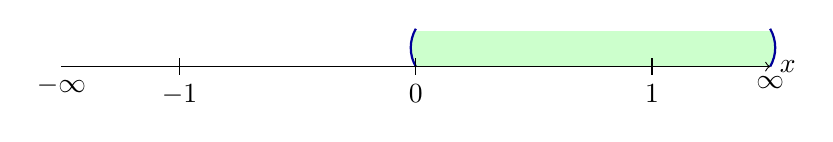
\begin{tikzpicture}[scale=3]
        %colores
        \colorlet{w}{green!20!white}
        \colorlet{bblue}{blue!60!black}

        % Figura relleno
        \fill[w](0,0) arc (210:150:1.5mm) -- +(1.5,0) arc (210:150:-1.5mm) -- cycle;
        % Parentesis, apertura, cierre
        \draw[bblue,thick](0,0) arc (210:150:1.6mm);
        \draw[bblue,thick](1.5,1.6mm) arc (210:150:-1.6mm);

        %Eje y numeracion
        \begin{scope}
            \draw[->] (-1.5,0) -- (1.5,0)node[right] {$x$}coordinate(x axis);
            \draw (-1.5,0) node[below] {$-\infty$}coordinate(x axis);
            \draw (1.5,0) node[below] {$\infty$}coordinate(x axis);
            \foreach \x/\xtext in {-1, 0, 1/-1,0,1}
            \draw[xshift=\x cm] (0pt,1pt) -- (0pt,-1pt) node[below,fill=white] {$\xtext$};
        \end{scope}
    \end{tikzpicture}

    para $ x \geq 0$

    Con circulo y flecha:

    \vspace*{1cm}
    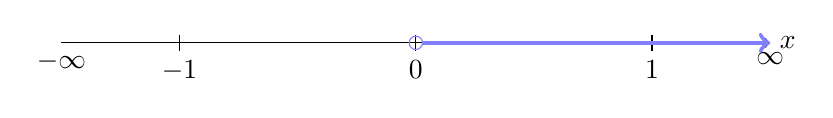
\begin{tikzpicture}[scale=3]
        \colorlet{w}{blue!50!white}
        \begin{scope}
            \draw[->] (-1.5,0) -- (1.5,0)node[right] {$x$}coordinate(x axis);
            \draw (-1.5,0) node[below] {$-\infty$}coordinate(x axis);
            \draw (1.5,0) node[below] {$\infty$}coordinate(x axis);
            \foreach \x/\xtext in {-1/-1, 0, 1/1}
            \draw[xshift=\x cm] (0pt,1pt) -- (0pt,-1pt) node[below,fill=white] {$\xtext$};
        \end{scope}
        \draw[w] (0,0) circle (0.8pt);
        \draw[w,ultra thick, ->] (0.8pt,0) -- (1.5,0);
    \end{tikzpicture}


    Si fuera $x\geq0$ lo único que cambiaría seria la parte de marca. Seria un
    corchete y un punto cerrado:

    Con corchete:

    %inmayore
    \vspace*{1cm}
    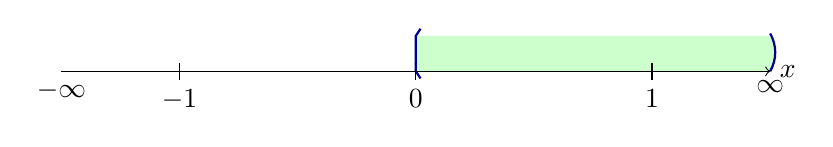
\begin{tikzpicture}[scale=3]
        %colores
        \colorlet{w}{green!20!white}
        \colorlet{bblue}{blue!60!black}

        % Figura relleno
        \fill[w](0,0) -- (0,1.5mm) -- +(1.5,0) arc (210:150:-1.5mm) -- cycle;
        % corchete, apertura, parentesis cierre
        \draw[bblue,thick](0,0) -- +(0.2mm, -0.3mm) (0,0)-- (0,1.5mm) -- +(0.2mm,0.3mm);
        \draw[bblue,thick](1.5,1.6mm) arc (210:150:-1.6mm);

        %Eje y numeracion
        \begin{scope}
            \draw[->] (-1.5,0) -- (1.5,0)node[right] {$x$}coordinate(x axis);
            \draw (-1.5,0) node[below] {$-\infty$}coordinate(x axis);
            \draw (1.5,0) node[below] {$\infty$}coordinate(x axis);
            \foreach \x/\xtext in {-1/-1, 0, 1/1}
            \draw[xshift=\x cm] (0pt,1pt) -- (0pt,-1pt) node[below,fill=white] {$\xtext$};
        \end{scope}
    \end{tikzpicture}


    Con punto y flecha:

    \vspace*{1cm}
    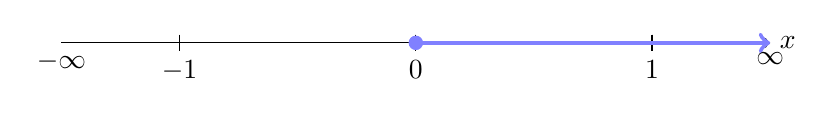
\begin{tikzpicture}[scale=3]
        \colorlet{w}{blue!50!white}
        \begin{scope}
            \draw[->] (-1.5,0) -- (1.5,0)node[right] {$x$}coordinate(x axis);
            \draw (-1.5,0) node[below] {$-\infty$}coordinate(x axis);
            \draw (1.5,0) node[below] {$\infty$}coordinate(x axis);
            \foreach \x/\xtext in {-1, 0, 1/-1,0,1}
            \draw[xshift=\x cm] (0pt,1pt) -- (0pt,-1pt) node[below,fill=white] {$\xtext$};
        \end{scope}
        \filldraw[w] (0,0) circle (0.8pt);
        \draw[w,ultra thick, ->] (0.8pt,0) -- (1.5,0);
    \end{tikzpicture}

    Es mas utilizado la primera forma (corchete y paréntesis) ya que facilita
    comparaciones en intervalos. Por esto, aunque ambos son equivalentes, de ahora
    en adelante se graficarán solamente estos.

    Otros ejemplos:

    $x<-5$
    puntos: -5 valor de la desigualdad, 0 e infinitos referencia.

    valores: tomamos un punto, ej 0 (esta a la derecha de -5 en la recta real)
    entonces: $x<-5,\ 0<-5$? no, no lo es, $0>-5$ y por ende es el otro lado de
    la recta la que cumple la desigualdad. El lado \textbf{izquierdo}.
    La gráfica es:

    %inmenor
    \vspace*{1cm}
    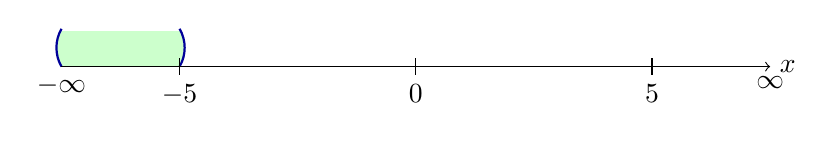
\begin{tikzpicture}[scale=3]
        %colores
        \colorlet{w}{green!20!white}
        \colorlet{bblue}{blue!60!black}

        % Figura relleno
        \fill[w](-1.5,0) arc (210:150:1.5mm) -- +(0.5,0) arc (210:150:-1.5mm) -- cycle;
        % Parentesis, apertura, cierre
        \draw[bblue,thick](-1.50,0) arc (210:150:1.6mm);
        \draw[bblue,thick](-1,1.6mm) arc (210:150:-1.6mm);

        %Eje y numeracion
        \begin{scope}
            \draw[->] (-1.5,0) -- (1.5,0)node[right] {$x$}coordinate(x axis);
            \draw (-1.5,0) node[below] {$-\infty$}coordinate(x axis);
            \draw (1.5,0) node[below] {$\infty$}coordinate(x axis);
            \foreach \x/\xtext in {-1/-5, 0, 1/5}
            \draw[xshift=\x cm] (0pt,1pt) -- (0pt,-1pt) node[below,fill=white] {$\xtext$};
        \end{scope}
    \end{tikzpicture}


    $x\leq -5$

    %inmenore
    \vspace*{1cm}
    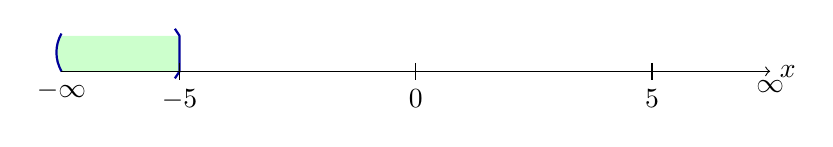
\begin{tikzpicture}[scale=3]
        %colores
        \colorlet{w}{green!20!white}
        \colorlet{bblue}{blue!60!black}

        % Figura relleno
        \fill[w](-1.5,0) arc (210:150:1.5mm) -- +(0.5,0) -- (-1,0) -- cycle;

        % parentesis, apertura, corchete cierre

        \draw[bblue,thick](-1.50,0) arc (210:150:1.6mm);
        \draw[bblue,thick](-1,1.5mm)-- +(-0.2mm,0.3mm) (-1,1.5mm)-- (-1,0)-- +(-0.2mm,-0.3mm);

        %Eje y numeracion
        \begin{scope}
            \draw[->] (-1.5,0) -- (1.5,0)node[right] {$x$}coordinate(x axis);
            \draw (-1.5,0) node[below] {$-\infty$}coordinate(x axis);
            \draw (1.5,0) node[below] {$\infty$}coordinate(x axis);
            \foreach \x/\xtext in {-1/-5, 0, 1/5}
            \draw[xshift=\x cm] (0pt,1pt) -- (0pt,-1pt) node[below,fill=white] {$\xtext$};
        \end{scope}
    \end{tikzpicture}

    \subsubsection{Tipos de inecuaciones} \label{Tipos-de-inecuaciones}

    Las inecuaciones al igual que las ecuaciones pueden ser clasificadas en
    distintos tipos, los mas comunes y relevantes son:

    \begin{itemize}
        \item Inecuaciones Lineales.
        \item Inecuaciones de grado $n$, $n \not = \{0,1\}$.
        \item Inecuaciones con valor absoluto.
        \item Inecuaciones racionales.
    \end{itemize}

    Esta clasificación se hace porque la forma de resolverla varia
    considerablemente para cada uno de estos.

    \subsubsection*{Inecuaciones Lineales} \label{Inecuaciones-Lineales}

    Las inecuaciones lineales son el equivalente a las ecuaciones algebraicas
    de grado 1, es decir, son la forma mas fácil de resolver y los ejemplos que
    se han dado hasta ahora son de este tipo. para resolver
    estas basta con despejar, de la forma explicada en \refname{ecuaciones},
    y tener en consideración la inversión de los operadores relacionales al
    multiplicar o dividir por un numero negativo. \textbf{RECUERDE que:}
    \textbf{cuando se despeja un numero negativo que multiplica
    o divide se invierte el operador relacional}.

    \textbf{Es importante saber } que en este tipo de inecuaciones siempre habrá
    un único conjunto solución.

    Ejemplos:

    \begin{align*}
        8x -45  &<9 		\\
        8x &< 9+45 \\
        8x & < 54\\
        x & < \frac{54}{8} \\
        x & < \frac{27}{4}
    \end{align*}

    Una vez completado el despeje, se procede a crear el conjunto y graficar:

    Punto único, $\displaystyle\frac{27}{4}$

    Tomando un valor, 0 por conveniencia, a la izquierda de $\displaystyle\frac{27}{4}$
    en la recta real,
    se tiene: $\displaystyle0<\frac{27}{4}$ ? si, entonces ese es el lado del intervalo que
    soluciona la inecuación.


    \textbf{El conjunto:} $\displaystyle\left(-\infty; \frac{27}{4}\right)$

    \textbf{La gráfica:}

    \vspace*{1cm}
    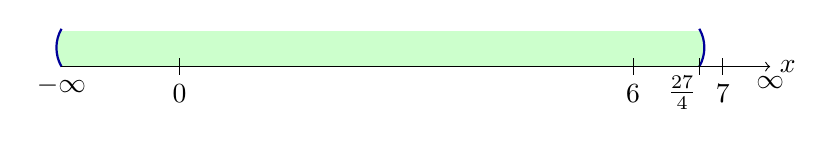
\begin{tikzpicture}[scale=3]
        %colores
        \colorlet{w}{green!20!white}
        \colorlet{bblue}{blue!60!black}

        % Figura relleno
        \fill[w](-1.5,0) arc (210:150:1.5mm) -- (1.2,1.5mm) arc (210:150:-1.5mm) -- cycle;
        % Parentesis, apertura, cierre
        \draw[bblue,thick](-1.50,0) arc (210:150:1.6mm);
        \draw[bblue,thick](1.2,1.6mm) arc (210:150:-1.6mm);

        %Eje y numeracion
        \begin{scope}
            \draw[->] (-1.5,0) -- (1.5,0)node[right] {$x$}coordinate(x axis);
            \draw (-1.5,0) node[below] {$-\infty$}coordinate(x axis);
            \draw (1.5,0) node[below] {$\infty$}coordinate(x axis);
            \foreach \x/\xtext in {-1/0, 0.92/6 ,1.2/  ,1.3/7}
            \draw[xshift=\x cm] (0pt,1pt) -- (0pt,-1pt) node[below] {$\xtext$};
        \end{scope}
        \draw (1.23,0) node[below left] {$\frac{27}{4} $};
    \end{tikzpicture}


    \begin{align*}
        9-45x \leq 639 		\\
        -45x \leq 639-9 \\
        -45x \leq 630 \\
        x \geq \frac{630}{-45} \\
        x \geq -14
    \end{align*}

    \textbf{nótese:} que como el despeje involucraba pasar de multiplicar a
    dividir un numero negativo, se invirtió el operador relacional ($\leq \Rightarrow \geq$)

    Una vez completado el despeje, se procede a crear el conjunto y graficar:

    Punto único, $-14$

    Tomando un valor, 0 por conveniencia, a la derecha de -14 en la recta real,
    se tiene: $0\geq -14$? si, entonces ese es el lado del intervalo que
    soluciona la inecuación.


    \textbf{El conjunto:} $[-14; \infty)$

    \textbf{La gráfica:}

    \vspace*{1cm}
    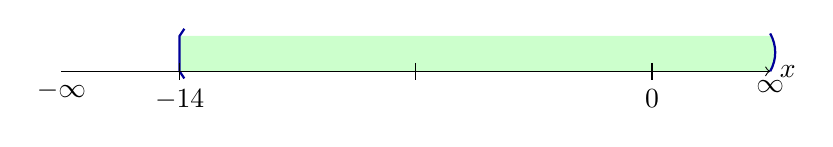
\begin{tikzpicture}[scale=3]
        %colores
        \colorlet{w}{green!20!white}
        \colorlet{bblue}{blue!60!black}

        % Figura relleno
        \fill[w](-1,0) -- (-1,1.5mm) -- (1.5,1.5mm) arc (210:150:-1.5mm) -- cycle;
        % corchete, apertura, parentesis cierre
        \draw[bblue,thick](-1,0) -- +(0.2mm, -0.3mm) (-1,0)-- (-1,1.5mm) -- +(0.2mm,0.3mm);
        \draw[bblue,thick](1.5,1.6mm) arc (210:150:-1.6mm);

        %Eje y numeracion
        \begin{scope}
            \draw[->] (-1.5,0) -- (1.5,0)node[right] {$x$}coordinate(x axis);
            \draw (-1.5,0) node[below] {$-\infty$}coordinate(x axis);
            \draw (1.5,0) node[below] {$\infty$}coordinate(x axis);
            \foreach \x/\xtext in {-1/-14, 0/ , 1/0}
            \draw[xshift=\x cm] (0pt,1pt) -- (0pt,-1pt) node[below,fill=white] {$\xtext$};
        \end{scope}
    \end{tikzpicture}



   \begin{align*}
       (95x -10)^3 &> 27		\\
       95x -10 &> \sqrt[3]{27} \\
       95x &> 3 +10\\
       x &> \frac{13}{95} \\
   \end{align*}

    Una vez completado el despeje, se procede a crear el conjunto y graficar:

    Punto único, $\displaystyle\frac{13}{95}$

    Tomando un valor, 0 por conveniencia, a la izquierda de $\displaystyle\frac{13}{95}$
    en la recta real,
    se tiene: $\displaystyle0 > \frac{13}{95} $ ? No, entonces ese no es el lado del intervalo que
    soluciona la inecuación, por lo tanto el lado solución es a la derecha de
    $\displaystyle\frac{13}{95}$.


    \textbf{El conjunto:} $\displaystyle\left(\frac{13}{95}; \infty\right)$

    \textbf{La gráfica:}

     \vspace*{1cm}
    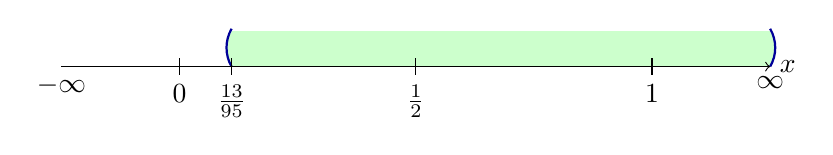
\begin{tikzpicture}[scale=3]
        %colores
        \colorlet{w}{green!20!white}
        \colorlet{bblue}{blue!60!black}

        % Figura relleno
        \fill[w](-0.78,0) arc (210:150:1.5mm) -- (1.5,1.5mm) arc (210:150:-1.5mm) -- cycle;
        % Parentesis, apertura, cierre
        \draw[bblue,thick](-0.78,0) arc (210:150:1.6mm);
        \draw[bblue,thick](1.5,1.6mm) arc (210:150:-1.6mm);

        %Eje y numeracion
        \begin{scope}
            \draw[->] (-1.5,0) -- (1.5,0)node[right] {$x$}coordinate(x axis);
            \draw (-1.5,0) node[below] {$-\infty$}coordinate(x axis);
            \draw (1.5,0) node[below] {$\infty$}coordinate(x axis);
            \foreach \x/\xtext in {-1/0,-0.78/\frac{13}{95} , 0/\frac{1}{2}  , 1/1}
            \draw[xshift=\x cm] (0pt,1pt) -- (0pt,-1pt) node[below,fill=white] {$\xtext$};
        \end{scope}
    \end{tikzpicture}


    \begin{align*}
        \frac{3x+1}{7} -\frac{2-4x}{3}  &\geq \frac{-5x-4}{14} + \frac{7x}{6} 		\\
        \text{M.C.M(7,3,14,6)=42, multiplicamos}& \text{ ambos lados para eliminar denominadores}\\
        42\times\left(\frac{3x+1}{7} -\frac{2-4x}{3}\right)  &\geq 42\times \left( \frac{-5x-4}{14} + \frac{7x}{6} \right)\\
        6(3x+1)-14(2-4x) &\geq 3(-5x-4) + 49x\\
        18x+6-28+56x &\geq -15x-12+49x\\
        18x+56x+15x-49x &\geq -12 -6 +28\\
        40x &\geq 10\\
        x &\geq \frac{10}{40} \\
        x &\geq \frac{1}{4}
    \end{align*}

    Una vez completado el despeje, se procede a crear el conjunto y graficar:

    Punto único, $\displaystyle\frac{1}{4}$

    Tomando un valor, 0 por conveniencia, a la izquierda de $\displaystyle\frac{1}{4}$
    en la recta real,
    se tiene: $\displaystyle0 \geq \frac{1}{4} $ ? No, entonces ese no es el lado del intervalo que
    soluciona la inecuación, por lo tanto el lado solución es a la derecha de
    $\displaystyle\frac{1}{4}$.


    \textbf{El conjunto:} $\displaystyle\left[\frac{1}{4}; \infty\right)$

    \textbf{La gráfica:}

    \vspace*{1cm}
    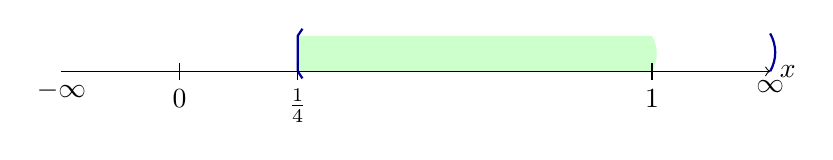
\begin{tikzpicture}[scale=3]
        %colores
        \colorlet{w}{green!20!white}
        \colorlet{bblue}{blue!60!black}

        % Figura relleno
        \fill[w](-0.5,0) -- (-0.5,1.5mm) -- +(1.5,0) arc (210:150:-1.5mm) -- cycle;
        % corchete, apertura, parentesis cierre
        \draw[bblue,thick](-0.5,0) -- +(0.2mm, -0.3mm) (-0.5,0)-- (-0.5,1.5mm) -- +(0.2mm,0.3mm);
        \draw[bblue,thick](1.5,1.6mm) arc (210:150:-1.6mm);

        %Eje y numeracion
        \begin{scope}
            \draw[->] (-1.5,0) -- (1.5,0)node[right] {$x$}coordinate(x axis);
            \draw (-1.5,0) node[below] {$-\infty$}coordinate(x axis);
            \draw (1.5,0) node[below] {$\infty$}coordinate(x axis);
            \foreach \x/\xtext in {-1/0,-0.5/\frac{1}{4},  1/1}
            \draw[xshift=\x cm] (0pt,1pt) -- (0pt,-1pt) node[below,fill=white] {$\xtext$};
        \end{scope}
    \end{tikzpicture}


\subsubsection*{Inecuaciones de grado $n$}
    Una inecuaciones de grado $n$, es el equivalente de las ecuaciones de grado
    2 hacia adelante (3,4,5,...) y la forma de resolverlas es distinta a las
    lineales. Esto es porque se generan mas de 1 punto que crea intervalos, mientras
    mayor sea el grado de la inecuación mayor puntos se dan y mayor sera la
    cantidad de \textbf{posibles intervalos solución}.

    Para resolver una inecuación de este estilo se deben encontrar todos los
    posibles intervalos y \textbf{unirlos} ($ A\cup B $)
    \textbf{intersectarlos} ($ A\cap B$)

    Para resolver este tipo de inecuaciones se deben seguir los siguientes pasos:

    \begin{itemize}
        \item Despejar la inecuación hasta igualar un extremo a 0 (forma canónica).
        \item Factorizar la ecuación para conseguir los puntos críticos o raíces
            de la ecuación.
        \item Graficar los puntos críticos y hallar los intervalos en los que
            la inecuación se cumpla.
        \item Formar los intervalos con los puntos críticos y respetando los
            operadores de relación.
    \end{itemize}

    Los puntos 3 y 4 se pueden invertir en orden, dependiendo de los gustos y las
    dificultades de cada quien puede ser mas sencillo primero graficar o primero
    encontrar los intervalos.

    Para realizar las gráficas, se debe graficar cada
    posible intervalo. Los posibles intervalos vienen dados por los puntos, raíces,
    de los \textbf{los elementos factorizados}. Cada uno de estos se observa como
    una inecuación nueva y se grafican, los intervalos solución vienen dados por
    los punto solución en los cuales se cumple la inecuación, estos puntos
    a su vez ya indican que tipo de relación guardan (paréntesis o corchetes),
    por lo tanto es fácil obtener la información.

    Para recordar como factorizar puede ir a \refname{Factorización}.

    Para proseguir, tomaremos las ecuaciones resueltas con anterioridad en
    \ref{Ecuaciones-2do-orden} y \ref{Ecuaciones-de-3er-orden-o-superior}
    y nos concentraremos en resolver los intervalos.

    Para: $x^2+5x-14 < 0$ factorizamos $x^2+5x-14 = 0$


    $$ x^2 + 5x -14 = 0$$
    $$ x_1 = 2\ ;\    x_2 = -7$$
    $$ x^2 + 5x -14 = 0 \longrightarrow  (x-2)(x+7) =0 $$

    Y la inecuación queda:

    $$ x^2 + 5x -14 < 0 \longrightarrow  (x-2)(x+7) < 0 $$

    cada factor se graficará independientemente, en la \textbf{raíz} como resultado
    de una inecuación lineal (la raíz es el valor
    que esta dentro del paréntesis pero con signo opuesto, ej para (x-2) seria
    x=2, esto sale del despeje... x-2=0 $\rightarrow$ x=2).


    Por facilidad, se busca que las gráficas tengan la misma referencia, y de ser
    posible la misma escala, para esto o se dibujan en la misma recta real o se hacen
    rectas reales iguales o centradas con respecto al 0, ya que este es referencia.

    Los puntos son: $ P_1 = 2\ ,\ P_2 =-7 $

    La gráfica de los puntos es::

    \vspace*{1cm}
    \begin{tikzpicture}[scale=1.5]
        %colores
        \colorlet{w}{green!20!white}
        \colorlet{bblue}{blue!60!black}

        % Figura relleno
        %\fill[w](-0.5,0) -- (-0.5,1.5mm) -- +(1.5,0) arc (210:150:-1.5mm) -- cycle;
        % Lineas verticales
        \draw[bblue,thick](-3.5,0)--(-3.5,0.5);
        \draw[bblue,thick](1,0) -- (1,0.5);

        %Eje y numeracion
        \begin{scope}
            \draw[->] (-5,0) -- (5,0)node[right] {$x$}coordinate(x axis);
            \draw (-5,0) node[below] {$-\infty$}coordinate(x axis);
            \draw (5,0) node[below] {$\infty$}coordinate(x axis);
            \foreach \x/\xtext in {-4/-8,-3.5/-7,-2/-4,0,1/2,2/4,4/8}
            \draw[xshift=\x cm] (0pt,1pt) -- (0pt,-1pt) node[below,fill=white] {$\xtext$};
        \end{scope}
    \end{tikzpicture}

    Dela gráfica se observan los intervalos (por las separaciones) $ \displaystyle
    (-\infty,-7);(-7,2);(2,+\infty)$


    Para saber si se cumple la inecuación en los intervalos, se elige un valor cualquiera
    que pertenezca al intervalo que se evalúa y se sustituye en la expresión.

    Tenemos:
    Intervalos: $ \displaystyle (-\infty,-7);(-7,2);(2,+\infty)$
    Inecuación: $ (x-2)(x+7) < 0 $
    Valores de muestra, pueden ser cualquiera:
    -8; 0; 8 (tomamos estos valores por facilidad, cada uno representa su intervalo)

    Sustituyendo:

    Para -8

    \begin{align*}
        (-8-2)(-8+7) & < 0  		\\
        (-10)(-1)   & < 0\\
        10 < 0
    \end{align*}
    Se observa que no pertenece el intervalo a la solución porque no cumple la inecuación.

    Para 0
    \begin{align*}
        (0-2)(0+7) & < 0  		\\
        (-2)(7)   & < 0\\
        -14 < 0
    \end{align*}
    Se observa que si cumple.

    Para 8
    \begin{align*}
        (8-2)(8+7) & < 0  		\\
        (6)(15)   & < 0\\
        90 < 0
    \end{align*}
    Se observa que no pertenece el intervalo a la solución.

    y de esta forma, el intervalo solución es $x\in(-7,2)$ y la gráfica es:

    \vspace*{1cm}
    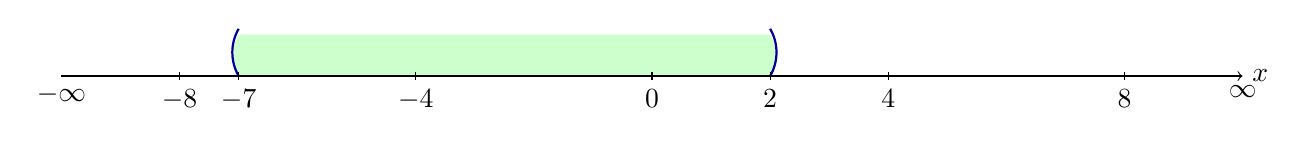
\begin{tikzpicture}[scale=1.5]
        %colores
        \colorlet{w}{green!20!white}
        \colorlet{bblue}{blue!60!black}

        % Figura relleno
        \fill[w] (-3.5,0) arc (210:150:0.35) --(1,0.35) arc (210:150:-0.35)--cycle ;
        % Parentesis, apertura, cierre
        \draw[bblue,thick](-3.5,0) arc (210:150:0.4);
        \draw[bblue,thick](1,0.4) arc (210:150:-0.4);

        %Eje y numeracion
        \begin{scope}
            \draw[->] (-5,0) -- (5,0)node[right] {$x$}coordinate(x axis);
            \draw (-5,0) node[below] {$-\infty$}coordinate(x axis);
            \draw (5,0) node[below] {$\infty$}coordinate(x axis);
            \foreach \x/\xtext in {-4/-8,-3.5/-7,-2/-4,0,1/2,2/4,4/8}
            \draw[xshift=\x cm] (0pt,1pt) -- (0pt,-1pt) node[below,fill=white] {$\xtext$};
        \end{scope}
    \end{tikzpicture}

    Esta forma de resolver es sencilla y practica, la mayor dificultad es las
    multiplicaciones. Cabe resaltar que \textbf{NO ES NECESARIO} hacer las
    multiplicaciones, ya que con el signo es suficiente. \textbf{Recordemos} que
    todo numero > o $\geq$ que 0 (cero) es positivo y en caso contrario, es
    < si es negativo o $ \leq $  si es negativo o 0.

    Se hace este énfasis por dos razones.

    \begin{itemize}
        \item Evitar cálculos innecesarios que pueden llevar mucho tiempo.
        \item Es la base del método de barras o tabla de signos, que es muy
            utilizado y sirve también para las inecuaciones racionales.
    \end{itemize}

   \subsubsection{Método de barras} \label{Metodo-de-barras}

   El método de barras o de tabla de signos consiste en hacer una tabla, colocar
   en la parte superior los intervalos posible solución, a la izquierda colocar
   todos los términos que impliquen una raíz. Es decir, \textbf{Todos los factores
   que se están multiplicando o dividiendo que son de la forma $(x\pm a) $},
   pueden convertir en 0 la multiplicación. Además, se coloca  un renglón adicional
   para la solución, usualmente al final como si fuera una multiplicación

   Posteriormente, se procede a rellenar la tabla con los signos resultantes en
   el intervalo, se toma un valor perteneciente al intervalo trabajado
   y se reemplaza en el monomio $(x\pm a) $, se coloca el signo. Luego se
   multiplican los signos de cada columna y el resultado se coloca en el renglón
   solución.

    El renglón solución indicara que valores toma la inecuación final y se observa
    si cumple con el operador relacional.

    \vspace*{1cm}
    \begin{tabular}{|c|c|}
        \hline
        Operador Relacional (inecuación)    &  Signo que lo satisface\\\hline
        $expresión<0 $                      &  negativo \n \\\hline
        $ expresión\leq0 $                  &  negativo \n \\\hline
        $expresión>0$                       &  positivo \p \\\hline
        $ expresión\geq0 $                  &  positivo \p \\\hline
    \end{tabular}

    \vspace*{1cm}
    Usando el mismo ejemplo anterior:

    Inecuación: $ (x-2)(x+7) < 0 $

    Intervalos: $ \displaystyle (-\infty,-7);(-7,2);(2,+\infty)$

    La tabla:

    \vspace*{1cm}
    \begin{tabular}{|c|c|c|c|}
              & $(-\infty,-7)$ & $(-7,2)$ & $(2,+\infty)$\\\hline
        $x-2$ &
        $x+7$ &
    Resultado &
    \end{tabular}

    \vspace*{1cm}
    Procedemos a llenar la tabla, calculando:
    para (x-2):

    -8: $ x-2 \rightarrow -8-2 \rightarrow -10 $ negativo

     0: $ x-2 \rightarrow 0-2 \rightarrow -2 $ negativo

    8: $ x-2 \rightarrow 8-2 \rightarrow 6 $ positivo

    para (x+7):

    -8: $ -8+7 \rightarrow -1 $ negativo

     0: $ 0+7 \rightarrow 7 $ positivo

    8: $ 8+7 \rightarrow 15 $ positivo

    \vspace*{1cm}
    \begin{tabular}{|c|c|c|c|}
        \hline
        binomio& \multicolumn{3}{c|}{Intervalos}\\
              & $(-\infty,-7)$ & $(-7,2)$ & $(2,+\infty)$\\\hline
        $x-2$ & \n &\n&\p \\\hline
        $x+7$ &\n &\p& \p \\\hline \hline
        Resultado & \p &\n&\p \\\hline
    \end{tabular}

    \vspace*{1cm}

    y de esta forma, el intervalo solución es $x\in(-7,2)$, ya que es el único
    negativo y por ende el único que cumple la inecuación y la gráfica es:

    \vspace*{1cm}
    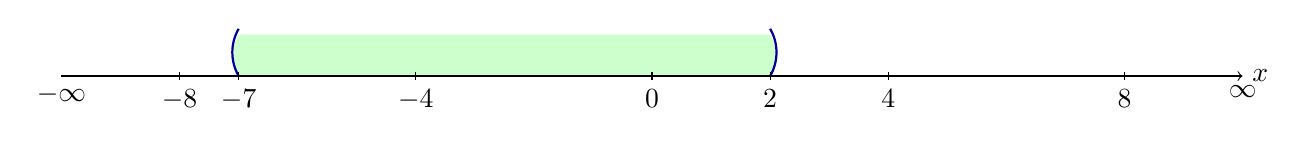
\begin{tikzpicture}[scale=1.5]
        %colores
        \colorlet{w}{green!20!white}
        \colorlet{bblue}{blue!60!black}

        % Figura relleno
        \fill[w] (-3.5,0) arc (210:150:0.35) --(1,0.35) arc (210:150:-0.35)--cycle ;
        % Parentesis, apertura, cierre
        \draw[bblue,thick](-3.5,0) arc (210:150:0.4);
        \draw[bblue,thick](1,0.4) arc (210:150:-0.4);

        %Eje y numeracion
        \begin{scope}
            \draw[->] (-5,0) -- (5,0)node[right] {$x$}coordinate(x axis);
            \draw (-5,0) node[below] {$-\infty$}coordinate(x axis);
            \draw (5,0) node[below] {$\infty$}coordinate(x axis);
            \foreach \x/\xtext in {-4/-8,-3.5/-7,-2/-4,0,1/2,2/4,4/8}
            \draw[xshift=\x cm] (0pt,1pt) -- (0pt,-1pt) node[below,fill=white] {$\xtext$};
        \end{scope}
    \end{tikzpicture}

    Ahora, estudiemos para el caso del operador relacional opuesto, para
    Inecuación: $ (x-2)(x+7) > 0 $

    El procedimiento es el mismo, y se llega a la misma tabla:

    \vspace*{1cm}
    \begin{tabular}{|c|c|c|c|}
        \hline
        binomio& \multicolumn{3}{c|}{Intervalos}\\
              & $(-\infty,-7)$ & $(-7,2)$ & $(2,+\infty)$\\\hline
        $x-2$ & \n &\n&\p \\\hline
        $x+7$ &\n &\p& \p \\\hline \hline
        Resultado & \p &\n&\p \\\hline
    \end{tabular}

    Mas ahora, como se tiene la expresión $ expresión > 0$ buscamos por
    \textbf{TODOS} los intervalos positivos, y se usa el operador de conjuntos
    unión ($ \cup $) para indicar que ambos satisfacen la inecuación.

    Entonces la gráfica resultante es:

    \vspace*{1cm}
    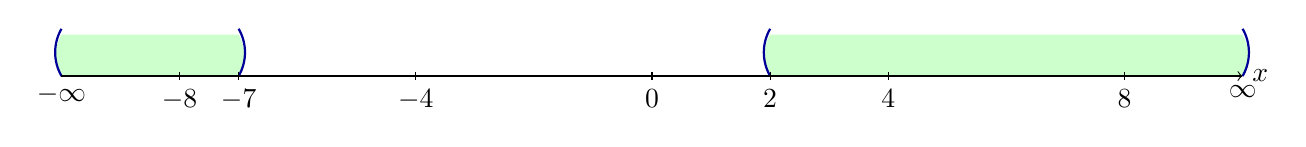
\begin{tikzpicture}[scale=1.5]
        %colores
        \colorlet{w}{green!20!white}
        \colorlet{bblue}{blue!60!black}

        % Figura relleno 1
        \fill[w] (-5,0) arc (210:150:0.35) --(-3.5,0.35) arc (210:150:-0.35)--cycle ;
        % Parentesis, apertura, cierre
        \draw[bblue,thick](-5,0) arc (210:150:0.4);
        \draw[bblue,thick](-3.5,0.4) arc (210:150:-0.4);

        % Figura relleno 2
        \fill[w] (1,0) arc (210:150:0.35) --(5,0.35) arc (210:150:-0.35)--cycle ;
        % Parentesis, apertura, cierre
        \draw[bblue,thick](1,0) arc (210:150:0.4);
        \draw[bblue,thick](5,0.4) arc (210:150:-0.4);

        %Eje y numeracion
        \begin{scope}
            \draw[->] (-5,0) -- (5,0)node[right] {$x$}coordinate(x axis);
            \draw (-5,0) node[below] {$-\infty$}coordinate(x axis);
            \draw (5,0) node[below] {$\infty$}coordinate(x axis);
            \foreach \x/\xtext in {-4/-8,-3.5/-7,-2/-4,0,1/2,2/4,4/8}
            \draw[xshift=\x cm] (0pt,1pt) -- (0pt,-1pt) node[below,fill=white] {$\xtext$};
        \end{scope}
    \end{tikzpicture}

    Y el conjunto solución es $x\in \{(-\infty;-7)\cup(2;+\infty) \} $.
    Se lee como, el conjunto formado por la unión de -infinito  a -7 con 2 a +infinito.


    \textbf{Además,} también se puede expresar como: $ \mathbb{R}-{[-7;2]} $, mas
    la otra nomenclatura es mas sencilla y se seguirá trabajando con esa. Notesé
    que en este caso los intervalos son cerrados, esto es porque ni -7 ni 2 pertenecen
    al intervalo solución, y por esto se deben añadir al conjunto exclusión.
    Esta nomenclatura se lee como, todos los reales excepto el conjunto de -7 a 2.

    Ahora procedamos con otro ejercicio, esta ecuación fue factorizada anteriormente
    en ecuaciones de 3er grado (\ref{Ecuaciones-de-3er-orden-o-superior})
    $ 2x^3+9x^2+13x = -6 \rightarrow (x+1)(x+2)\left(x+\frac{3}{2}\right) =  0  $

    Tomando la Factorización y resolviéndola para los 2 operadores relacionales
    que nos faltan por ver ( $ \leq,\geq $  ), tenemos:

    Para: $ (x+1)(x+2)\left(x+\frac{3}{2}\right) \leq 0 $

    Los puntos críticos son: -2,$ -\frac{3}{2}$(-1.5),-1 por ende, los intervalos
    son:
    $$\displaystyle (-\infty;-2], [-2;-\frac{3}{2}],[-\frac{3}{2},-1],  [-1,+\infty) $$

    Luego procedemos a tomar valores para cada intervalo:
    $ v_1=-3,v_2= -1.6,v_3= -1.1,v_4= 0 $

    Para (x+1):

    -3: -3+1=-2 negativo

    -1.6: -1.6+1=-0.6 negativo

    -1.1: -1.1+1=-0.1 negativo

    0: 0+1=1 positivo

    Para $\left(x+\frac{3}{2}\right)$:

    -3: $-3+\frac{3}{2}$=-$\frac{3}{2} $ negativo

    -1.6: $-1.6+\frac{3}{2}$=-0.1 negativo

    -1.1: $-1.1+\frac{3}{2}$=+0.4 positivo

    0: $0+\frac{3}{2}$=1.5 positivo

    Para (x+2):

    -3: -3+2=-1 negativo

    -1.6: -1.6+2=0.4 positivo

    -1.1: -1.1+2=0.9 positivo

    0: 0+2=2 positivo


    \vspace*{1cm}
    \begin{tabular}{|c|c|c|c|c|}
        \hline
        binomio& \multicolumn{4}{c|}{Intervalos}\\
              & $(-\infty;-2]$ & $ [-2;-\frac{3}{2}]$ & $[-\frac{3}{2},-1]$&$ [-1,+\infty)$\\\hline
        $x+1$ & \n &\n&\n&\p \\\hline
        $\left(x+\frac{3}{2}\right)$&\n&\n&\p&\p\\\hline
        $x+2$ &\n &\p& \p &\p \\\hline
        Resultado&\n & \p &\n&\p \\\hline
    \end{tabular}
    \vspace*{1cm}

    Y el conjunto solución es $x\in\{ (-\infty;-2]\cup \displaystyle \left[-\frac{3}{2},-1\right]\}  $
    (negativos).

    \vspace*{1cm}
    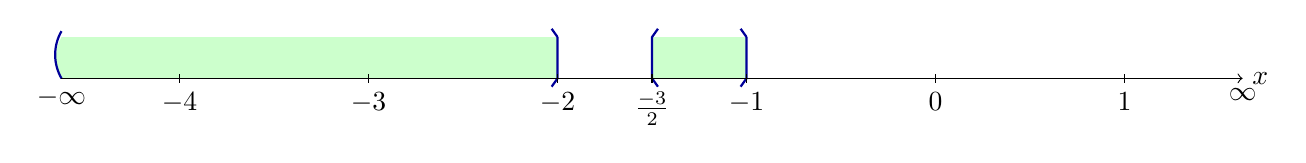
\begin{tikzpicture}[scale=1.5]
        %colores
        \colorlet{w}{green!20!white}
        \colorlet{bblue}{blue!60!black}

        % Figura relleno 1
        \fill[w] (-5,0) arc (210:150:0.35) --(-0.8,0.35) -- (-0.8,0) --cycle ;
        % Parentesis, apertura, corchete cierre
        \draw[bblue,thick](-5,0) arc (210:150:0.4);
        \draw[bblue,thick](-0.8,0.35)-- +(-0.5mm,0.7mm) (-0.8,0.35)-- (-0.8,0)-- +(-0.5mm,-0.7mm);


        % Figura relleno 2
        \fill[w] (0,0) rectangle  (0.8,0.35);
        % Corchete, apertura, cierre
        \draw[bblue,thick](0,0) -- +(0.5mm, -0.7mm) (0,0)-- (0,0.35) -- +(0.5mm,0.7mm);
        \draw[bblue,thick](0.8,0.35)-- +(-0.5mm,0.7mm) (0.8,0.35)-- (0.8,0)-- +(-0.5mm,-0.7mm);

        %Eje y numeracion
        \begin{scope}
            \draw[->] (-5,0) -- (5,0)node[right] {$x$}coordinate(x axis);
            \draw (-5,0) node[below] {$-\infty$}coordinate(x axis);
            \draw (5,0) node[below] {$\infty$}coordinate(x axis);
            \foreach \x/\xtext in {-4/-4,-2.4/-3,-0.8/-2,0/\frac{-3}{2} ,0.8/-1,2.4/0,4/1}
            \draw[xshift=\x cm] (0pt,1pt) -- (0pt,-1pt) node[below] {$\xtext$};
        \end{scope}
    \end{tikzpicture}



    Para: $ (x+1)(x+2)\left(x+\frac{3}{2}\right) \geq 0 $

    Tenemos lo mismo, por tanto llegamos a la tabla:

     \vspace*{1cm}
    \begin{tabular}{|c|c|c|c|c|}
        \hline
        binomio& \multicolumn{4}{c|}{Intervalos}\\
              & $(-\infty;-2]$ & $ [-2;-\frac{3}{2}]$ & $[-\frac{3}{2},-1]$&$ [-1,+\infty)$\\\hline
        $x+1$ & \n &\n&\n&\p \\\hline
        $\left(x+\frac{3}{2}\right)$&\n&\n&\p&\p\\\hline
        $x+2$ &\n &\p& \p &\p \\\hline
        Resultado&\n & \p &\n&\p \\\hline
    \end{tabular}
    \vspace*{1cm}

    Y el conjunto solución es $x\in \{ \displaystyle \left[-2;\frac{-3}{2}\right] \cup [-1,+\infty) \} $
    (positivos).

    La gráfica resultante es:

    \vspace*{1cm}
    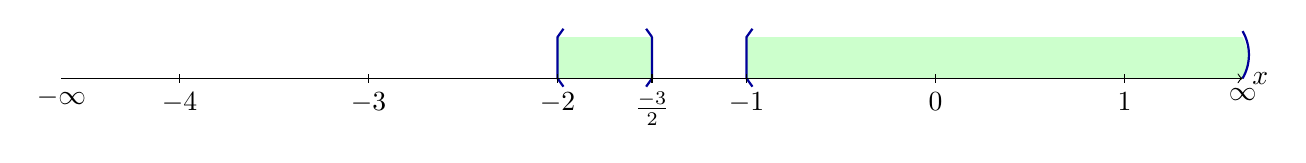
\begin{tikzpicture}[scale=1.5]
        %colores
        \colorlet{w}{green!20!white}
        \colorlet{bblue}{blue!60!black}

        % Figura relleno 1
        \fill[w] (-0.8,0) rectangle  (0,0.35);
        % corchete , apertura, cierre
        \draw[bblue,thick](-0.8,0) -- +(0.5mm, -0.7mm) (-0.8,0)-- (-0.8,0.35) -- +(0.5mm,0.7mm);
        \draw[bblue,thick](0,0.35)-- +(-0.5mm,0.7mm) (0,0.35)-- (0,0)-- +(-0.5mm,-0.7mm);


        % Figura relleno 2
        \fill[w] (0.8,0) -- (0.8,0.35) --  (5,0.35) arc (210:150:-0.35)--cycle ;
        % Corchete, apertura, parentesis cierre
        \draw[bblue,thick](0.8,0) -- +(0.5mm, -0.7mm) (0.8,0)-- (0.8,0.35) -- +(0.5mm,0.7mm);
        \draw[bblue,thick](5,0.4) arc (210:150:-0.4);

        %Eje y numeracion
        \begin{scope}
            \draw[->] (-5,0) -- (5,0)node[right] {$x$}coordinate(x axis);
            \draw (-5,0) node[below] {$-\infty$}coordinate(x axis);
            \draw (5,0) node[below] {$\infty$}coordinate(x axis);
            \foreach \x/\xtext in {-4/-4,-2.4/-3,-0.8/-2,0/\frac{-3}{2} ,0.8/-1,2.4/0,4/1}
            \draw[xshift=\x cm] (0pt,1pt) -- (0pt,-1pt) node[below] {$\xtext$};
        \end{scope}
    \end{tikzpicture}


\subsubsection*{Inecuaciones Racionales}
    Este tipo de inecuaciones tienen la forma $ \displaystyle \frac{P(x)}{Q(X)} $
    como una de las expresiones y el otro lado esta igualado a 0.
    $ P(x), Q(x) $ son expresiones algebraicas como las que hemos venido trabajando
    y la forma de resolución de estos es con el método de barras (tabla de signos),
    con algunas consideraciones adicionales:

    \begin{itemize}
        \item Se factorizar tanto numerador como denominador y se colocan los
            intervalos correspondientes
        \item El polinomio denominador \textbf{NO} puede ser 0, ya que la división
            por 0 no existe, por esto esos intervalos siempre serán \textbf{ABIERTOS},
            es decir, con un paréntesis "(" o ")" dependiendo si  es apertura o
            cierre del intervalo.
    \end{itemize}

    Ejemplos:

    Para $ \frac{x^2+x-2}{x} \geq 0 $
    Primero factorizados tanto numerador como denominador:
    Numerador:
    \begin{align*}
        x^2+x-2 &=0.\ a=1,b=1,c=-2 		\\
        x &= \frac{-1\pm \sqrt{1^2-4\times1\times-2}}{2\times1}\\
        \text{Al resolver se obtiene: }& x_1=1,\ x_2=-2\\
        \rightarrow (x-1)(x+2)&=0
    \end{align*}
    Denominador: $x$

    Y la inecuación factorizada queda de la forma:

    $$ \frac{(x-1)(x+2)}{x} \geq 0  $$

    Las raíces, puntos críticos, son: 1, -2, 0. Dando origen a los intervalos:
    $ (-\infty;-2]$, $[-2,0)$, $ (0,1] $, $[1,+\infty)$
    nótese que los intervalos son \textbf{ABIERTOS} en 0, esto es porque si el
    denominador se hace 0 (único punto en 0), la inecuación no existe y en los
    infinitos, porque estos se desconocen y por ende no se pueden tomar (misma
    razón que antes, por eso siempre es abierto en estos "puntos").

    De igual forma, procedemos a tomar valores entre los intervalos:
    -3,-1,0.5,2 por facilidad de los cálculos. entonces tenemos:

    Para (x-1):
    -3 : -3-1 = -4 negativo\\
    -1 : -1-1 = -2 negativo\\
    0.5 : 0.5-1 = -0.5 negativo\\
    2  : 2-1 = 1 positivo\\

    Para (x+2):
    -3 : -3+2 = -1 negativo\\
    -1 : -1+2 = 1 positivo\\
    -0.5 : -0.5+2 = 1.5 positivo \\
    2 : 2+2 = 4 positivo\\

    para x:
    -3 : -3 negativo\\
    -1 : -1 negativo\\
    0.5 : 0.5 positivo\\
    2 : 2 positivo\\

\vspace*{1cm}
    \begin{tabular}{|c|c|c|c|c|}
        \hline
            &$ (-\infty;-2]$&   $[-2,0)$ &$ (0,1] $ &$[1,+\infty)$\\\hline
        x-1 &  \n   & \n    & \n    & \p \\\hline
        x+2 & \n    & \p    & \p    & \p \\\hline
        x   & \n    & \n    & \p    & \p \\\hline
    resultado& \n   & \p    & \n    & \p \\\hline
    \end{tabular}
    \vspace*{1cm}

    De lo que se obtiene el intervalo resultado:$ \{x\in  [-2,0) \cup [1,+\infty) \}$

    Y la gráfica es:

 \vspace*{1cm}
    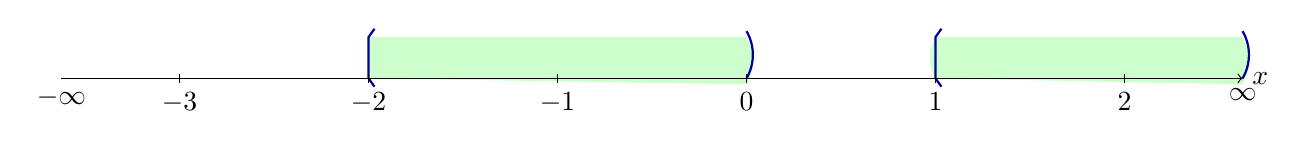
\begin{tikzpicture}[scale=1.5]
        %colores
        \colorlet{w}{green!20!white}
        \colorlet{bblue}{blue!60!black}

        % Figura relleno 1
        \fill[w] (-2.4,0)-- (-2.4,0.35)--(0.8,0.35) arc (210:150:-0.4);
        % Corchete, apertura, parentesis cierre
        \draw[bblue,thick](-2.4,0) -- +(0.5mm, -0.7mm) (-2.4,0)-- (-2.4,0.35) -- +(0.5mm,0.7mm);
        \draw[bblue,thick](0.8,0.4) arc (210:150:-0.4);

        % Figura relleno 2
        \fill[w] (2.4,0) arc (210:150:0.35) --(5,0.35) arc (210:150:-0.4) --cycle ;
        % corchete apertura, parentesis cierre
        \draw[bblue,thick](2.4,0) -- +(0.5mm, -0.7mm) (2.4,0)-- (2.4,0.35) -- +(0.5mm,0.7mm);
        \draw[bblue,thick](5,0.4) arc (210:150:-0.4);



        %Eje y numeracion
        \begin{scope}
            \draw[->] (-5,0) -- (5,0)node[right] {$x$}coordinate(x axis);
            \draw (-5,0) node[below] {$-\infty$}coordinate(x axis);
            \draw (5,0) node[below] {$\infty$}coordinate(x axis);
            \foreach \x/\xtext in {-4/-3,-2.4/-2,-0.8/-1,0.8/0,2.4/1,4/2}
            \draw[xshift=\x cm] (0pt,1pt) -- (0pt,-1pt) node[below] {$\xtext$};
        \end{scope}
    \end{tikzpicture}


    Otro ejemplo y un truco:
    \textbf{Si se sigue un orden creciente, una vez se presenta el cambio de
    signo, para un monomio, todos los posteriores tendrán el nuevo signo}

    $$ \frac{(x+1)(x+3)(x-3)}{(x-5)x} \leq 0$$

    Primero conseguimos los puntos críticos, raíces, estos son:

    Numerador:-1,-3,3, en orden creciente, -3,-1,3

    denominador:5,0 en orden creciente, 0,5

    Por lo tanto, los puntos son -3,-1,0,3,5 y los intervalos son:

    $ (-\infty,-3];[-3,-1];[-1,0);(0,3];[3,5);(5,+\infty) $

    Tomando puntos, estos serian, -4,-2,-0.5,1,4,6 y probando:\\

    Para (x+1):\\
    -4 : -4+1=-3, negativo \\
    -2 : -2+1 = -1, negativo\\
    -0.5 : -0.5+1=0.5 positivo \textbf{cambio de signo}\\
    1 : 1+1= 2 positivo\\
    4 : 4+1 = 5 positivo\\
    6 : 6+1=7 positivo \\

    Para (x+3):\\
    -4 :-4+3=-1 negativo\\
    -2 : -2+3 = 1 positivo \textbf{cambio de signo}\\
    -0.5 : -0.5 +3 = 2.5 positivo\\
    1 : 1+3 = 4 positivo\\
    4 : 4+3 = 7 positivo\\
    6 : 6+4 = 10 positivo\\

    Para (x-3):\\
    -4 : -4-3 =-7 negativo\\
    -2 : -2-3 =-5 negativo\\
    -0.5 : -0.5-3 =-3.5 negativo\\
    1 : 1-3=-2 negativo\\
    4 : 4-3=1 positivo \textbf{cambio de signo}\\
    6 : 6-3=3 positivo\\

    Para x:\\
    -4 : -4 negativo\\
    -2 : -2 negativo\\
    -0.5 : -0.5 negativo\\
    1 : 1 positivo  \textbf{cambio de signo}\\
    4 : positivo\\
    6 : positivo\\

    Para (x-5):\\
    -4 : -4-5 =-9 negativo\\
    -2 : -2-5 = -7 negativo\\
    -0.5 : -0.5-5=-5.5 negativo\\
    1 : 1-5 =-4 negativo\\
    4 : 4-5=-1 negativo \\
    6 : 6-5 = 1 positivo\\


\vspace*{1cm}
    \begin{tabular}{|c|c|c|c|c|c|c|}
        \hline
            &$ (-\infty,-3]$&   $[-3,-1]$ &$ [-1,0) $ &$(0,3]$& $ [3,5) $& $(5,+\infty)$\\\hline
        x+1 &  \n   & \n    & \p    & \p    & \p    & \p \\\hline
        x-3 & \n    & \n    & \n    & \n    & \p    & \p \\\hline
        x+3 & \n    & \p    & \p    & \p    & \p    & \p \\\hline
        x   & \n    &  \n   & \n    & \p    & \p    & \p \\\hline
        x-5 & \n    &  \n   & \n    & \n    & \n    & \p \\\hline
    resultado& \n   & \p    & \n    & \p    & \n    & \p \\\hline
    \end{tabular}
    \vspace*{1cm}

    El intervalo solución es: $x \in \{ (-\infty,-3]\cup[-1,0)\cup[3,5)  \}$


 \vspace*{1cm}
    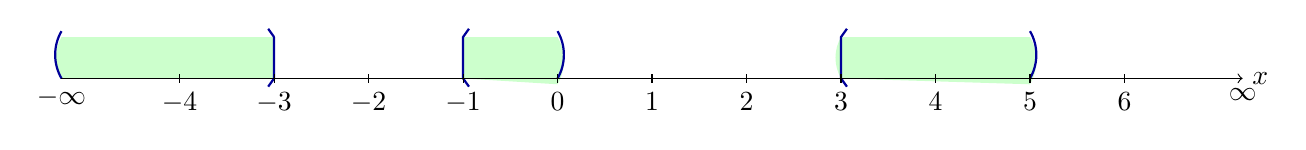
\begin{tikzpicture}[scale=1.5]
        %colores
        \colorlet{w}{green!20!white}
        \colorlet{bblue}{blue!60!black}
        % Figura relleno 1
        \fill[w] (-5,0) arc (210:150:0.35) --(-3.2,0.35) -- (-3.2,0) --cycle ;
        % Parentesis, apertura, corchete cierre
        \draw[bblue,thick](-5,0) arc (210:150:0.4);
        \draw[bblue,thick](-3.2,0.35)-- +(-0.5mm,0.7mm) (-3.2,0.35)-- (-3.2,0)-- +(-0.5mm,-0.7mm);

        % Figura relleno 2
        \fill[w] (-1.6,0)-- (-1.6,0.35)--(-0.8,0.35) arc (210:150:-0.4);
        % Corchete, apertura, parentesis cierre
        \draw[bblue,thick](-1.6,0) -- +(0.5mm, -0.7mm) (-1.6,0)-- (-1.6,0.35) -- +(0.5mm,0.7mm);
        \draw[bblue,thick](-0.8,0.4) arc (210:150:-0.4);

        % Figura relleno 3
        \fill[w] (1.6,0) arc (210:150:0.35) --(3.2,0.35) arc (210:150:-0.4) --cycle ;
        % corchete apertura, parentesis cierre
        \draw[bblue,thick](1.6,0) -- +(0.5mm, -0.7mm) (1.6,0)-- (1.6,0.35) -- +(0.5mm,0.7mm);
        \draw[bblue,thick](3.2,0.4) arc (210:150:-0.4);


        %Eje y numeracion
        \begin{scope}
            \draw[->] (-5,0) -- (5,0)node[right] {$x$}coordinate(x axis);
            \draw (-5,0) node[below] {$-\infty$}coordinate(x axis);
            \draw (5,0) node[below] {$\infty$}coordinate(x axis);
            \foreach \x/\xtext in {-4/-4,-3.2/-3,-2.4/-2,-1.6/-1,-0.8/0,0/1,0.8/2,1.6/3,2.4/4,3.2/5,4/6}
            \draw[xshift=\x cm] (0pt,1pt) -- (0pt,-1pt) node[below] {$\xtext$};
        \end{scope}
    \end{tikzpicture}

\subsubsection*{Inecuaciones con valor absoluto}

    Las inecuaciones con valor absoluto son bastante comunes, y se resuelven de
    una forma diferente a lo estudiado anteriormente. Para resolverlas se utiliza
    la definición de valor absoluto.

    \textbf{Recordemos: } que el valor absoluto, también conocido como modulo de
    un numero real, se escribe $|x|$ es el valor no negativo de la expresión $x$.
    Y se define como:

\begin{align*}
    |x| &=
    \left\lbrace
    \begin{array}{c}
        x, \text{ si }x \geq0\\
        -x, \text{ si }x < 0
    \end{array}
    \right.
\end{align*}


    Para resolver las inecuaciones con valor absoluto, debemos entonces, resolver
    primero el valor absoluto, luego resolver las inecuaciones resultantes y
    finalmente conseguir los intervalos que la satisfacen.

    Ejemplos:

    Cuando el operador es < o $\leq$, los intervalos se conectan:

\begin{align*}
    |x| &<K \rightarrow
    \left\lbrace
    \begin{array}{c}
        x, \text{ si }x \geq0\\
        -x, \text{ si }x < 0
    \end{array}
    \right.\\
    \text{Resolviendo tenemos }& \text{las inecuaciones:}  \\
    x < K\ &; \ -x < K\\
    x < K\ &; \  x > -K\\
    \text{Y el resultado se escribe }& \text{de la siguiente forma:}\\
    -K < x < K\ o&\ x\in (-k;k)
\end{align*}

    y la gráfica resultante es:

% inmayor
    \vspace*{1cm}
    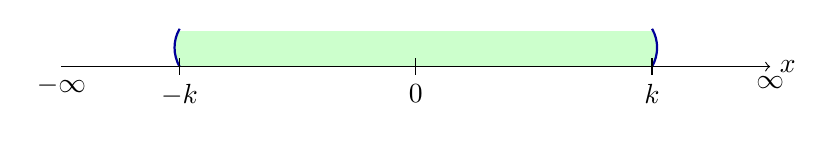
\begin{tikzpicture}[scale=3]
        %colores
        \colorlet{w}{green!20!white}
        \colorlet{bblue}{blue!60!black}

        % Figura relleno
        \fill[w](-1,0) arc (210:150:1.5mm) -- (1,1.5mm) arc (210:150:-1.5mm) -- cycle;
        % Parentesis, apertura, cierre
        \draw[bblue,thick](-1,0) arc (210:150:1.6mm);
        \draw[bblue,thick](1,1.6mm) arc (210:150:-1.6mm);

        %Eje y numeracion
        \begin{scope}
            \draw[->] (-1.5,0) -- (1.5,0)node[right] {$x$}coordinate(x axis);
            \draw (-1.5,0) node[below] {$-\infty$}coordinate(x axis);
            \draw (1.5,0) node[below] {$\infty$}coordinate(x axis);
            \foreach \x/\xtext in {-1/-k, 0/0, 1/k}
            \draw[xshift=\x cm] (0pt,1pt) -- (0pt,-1pt) node[below,fill=white] {$\xtext$};
        \end{scope}
    \end{tikzpicture}

    Como se observa, solo se aplica la definición y se procede a resolver las
    inecuaciones por separado.

    algunos ejemplos mas complejos serian:

\begin{align*}
    |x-5| &\leq3 \rightarrow
    \left\lbrace
    \begin{array}{c}
        x-5, \text{ si }x \geq0\\
        -x-(-5)= 5-x, \text{ si }x < 0
    \end{array}
    \right.\\
\end{align*}
    Resolviendo tenemos las inecuaciones:  \\

\begin{align*}
    x-5 & \leq 3    &  5-x &\leq 3	\\
    x &\leq 3+5     &  -x &\leq 3-5 \\
    x & \leq 8      &  -x &\leq -2 \\
    x& \leq 8       &   x &\geq 2
\end{align*}

    y se tiene el intervalo:
    $2\leq x\leq8$ o, de la otra forma, $x \in [2;8]$

    Y la gráfica resultante es:

 \vspace*{1cm}
    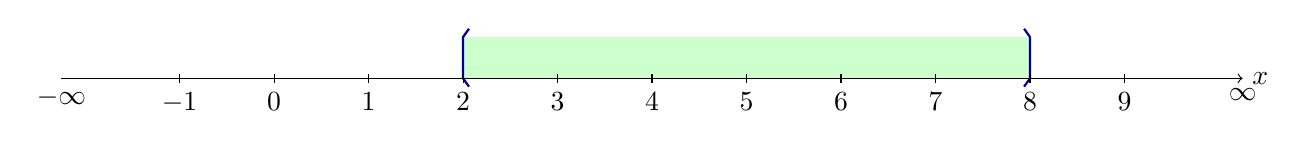
\begin{tikzpicture}[scale=1.5]
        %colores
        \colorlet{w}{green!20!white}
        \colorlet{bblue}{blue!60!black}
        % Figura relleno 1
        \fill[w] (-1.6,0)-- (-1.6,0.35)--(3.2,0.35) -- (3.2,0) --cycle ;
        %  corchete , apertura,cierre
        \draw[bblue,thick](-1.6,0) -- +(0.5mm, -0.7mm) (-1.6,0)-- (-1.6,0.35) -- +(0.5mm,0.7mm);
        \draw[bblue,thick](3.2,0.35)-- +(-0.5mm,0.7mm) (3.2,0.35)-- (3.2,0)-- +(-0.5mm,-0.7mm);


        %Eje y numeracion
        \begin{scope}
            \draw[->] (-5,0) -- (5,0)node[right] {$x$}coordinate(x axis);
            \draw (-5,0) node[below] {$-\infty$}coordinate(x axis);
            \draw (5,0) node[below] {$\infty$}coordinate(x axis);
            \foreach \x/\xtext in {-4/-1,-3.2/0,-2.4/1,-1.6/2,-0.8/3,0/4,0.8/5,1.6/6,2.4/7,3.2/8,4/9}
            \draw[xshift=\x cm] (0pt,1pt) -- (0pt,-1pt) node[below] {$\xtext$};
        \end{scope}
    \end{tikzpicture}

    Cuando el operador relacional es > o $\geq$, los intervalos son separados:

\begin{align*}
    |x| &>K \rightarrow
    \left\lbrace
    \begin{array}{c}
        x, \text{ si }x \geq0\\
        -x, \text{ si }x < 0
    \end{array}
    \right.\\
    \text{Resolviendo tenemos }& \text{las inecuaciones:}  \\
    x > K\ &; \ -x > K\\
    x > K\ &; \  x < -K\\
    \text{Y el resultado se escribe }& \text{de la siguiente forma:}\\
    x \in \{(-\infty;-K) \cup (K;\infty)\}
\end{align*}

Y la gráfica es:

\vspace*{1cm}
    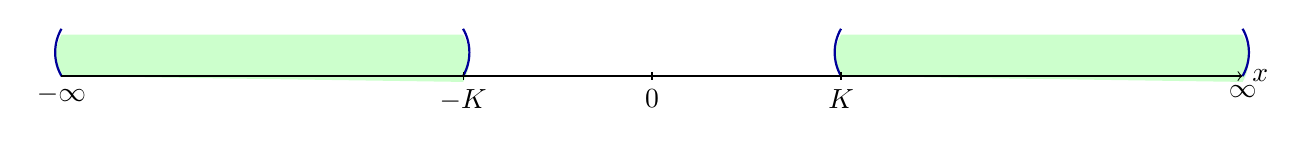
\begin{tikzpicture}[scale=1.5]
        %colores
        \colorlet{w}{green!20!white}
        \colorlet{bblue}{blue!60!black}
        % Figura relleno 1
        \fill[w] (-5,0) arc (210:150:0.35) --(-1.6,0.35)arc (210:150:-0.4) --cycle ;
        % Parentesis, apertura, cierre
        \draw[bblue,thick](-5,0) arc (210:150:0.4);
        \draw[bblue,thick](-1.6,0.4) arc (210:150:-0.4);

        % Figura relleno 2
        \fill[w] (1.6,0) arc (210:150:0.35)--(5,0.35) arc (210:150:-0.4)--cycle;
        % Corchete, apertura, parentesis cierre
        \draw[bblue,thick](1.6,0) arc (210:150:0.4);
        \draw[bblue,thick](5,0.4) arc (210:150:-0.4);

        %Eje y numeracion
        \begin{scope}
            \draw[->] (-5,0) -- (5,0)node[right] {$x$}coordinate(x axis);
            \draw (-5,0) node[below] {$-\infty$}coordinate(x axis);
            \draw (5,0) node[below] {$\infty$}coordinate(x axis);
            \foreach \x/\xtext in {-1.6/-K,0/0,1.6/K}
            \draw[xshift=\x cm] (0pt,1pt) -- (0pt,-1pt) node[below] {$\xtext$};
        \end{scope}
    \end{tikzpicture}

    Otro ejemplo:

\begin{align*}
    |x-1| &\geq 2x \rightarrow
    \left\lbrace
    \begin{array}{c}
        x-1, \text{ si }x \geq0\\
        -x-(-1)= 1-x, \text{ si }x < 0
    \end{array}
    \right.\\
\end{align*}

    Resolviendo tenemos las inecuaciones:
\begin{align*}
    x-1 & \geq 2x       &  1-x &\leq 2x	\\
    x -2x &\geq 1       &  -x-2x &\leq -1 \\
    -x & \geq 1         &  -3x &\leq -1 \\
    x&\leq -1           &   x &\geq \frac{-1}{-3}  \\
        &               &   x &\geq \frac{1}{3}
\end{align*}

y el intervalo solución es
$\displaystyle x \in \left\{ (-\infty;-1] \cup \left[\frac{1}{3};\infty\right) \right\}$

Y la gráfica es:

\vspace*{1cm}
    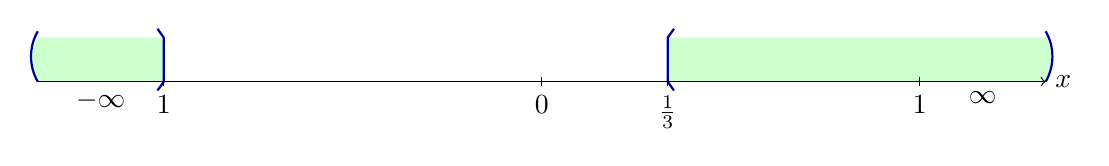
\begin{tikzpicture}[scale=1.6]
        %colores
        \colorlet{w}{green!20!white}
        \colorlet{bblue}{blue!60!black}
        % Figura relleno 1
        \fill[w] (-4,0) arc (210:150:0.35) --(-3,0.35)-- (-3,0) --cycle ;
        % Parentesis, apertura, cierre
        \draw[bblue,thick](-4,0) arc (210:150:0.4);
        \draw[bblue,thick](-3,0.35)-- +(-0.5mm,0.7mm) (-3,0.35)-- (-3,0)-- +(-0.5mm,-0.7mm);

        % Figura relleno 2
        \fill[w] (1,0) -- (1,0.35)--(4,0.35) arc (210:150:-0.35)--cycle;
        % Corchete, apertura, parentesis cierre
        \draw[bblue,thick](1,0) -- +(0.5mm, -0.7mm) (1,0)-- (1,0.35) -- +(0.5mm,0.7mm);
        \draw[bblue,thick](4,0.4) arc (210:150:-0.4);

        %Eje y numeracion
        \begin{scope}
            \draw[->] (-4,0) -- (4,0)node[right] {$x$}coordinate(x axis);
            \draw (-3.5,0) node[below] {$-\infty$}coordinate(x axis);
            \draw (3.5,0) node[below] {$\infty$}coordinate(x axis);

            \foreach \x/\xtext in {-3/1,0/0,1/\frac{1}{3},3/1}
            \draw[xshift=\x cm] (0pt,1pt) -- (0pt,-1pt) node[below] {$\xtext$};
        \end{scope}
    \end{tikzpicture}

    Otro ejemplo:

\begin{align*}
    \frac{|x+1|}{x}  &\geq 0  \rightarrow
    \left\lbrace
    \begin{array}{c}
        x + 1, \text{ si }x \geq0\\
        -x -1, \text{ si }x < 0
    \end{array}
    \right.\\
\end{align*}

    Para que la inecuación se cumpla, se tiene que cumplir que $ \frac{a}{b} \geq 0 $
    Como el numerador siempre dará un resultado positivo (por eso tiene el valor
    absoluto), lo único que puede modificar el resultado es el denominador, entonces
    el intervalo estará dictado por que $ den \geq 0 $

    $ x\geq 0 \rightarrow$ el intervalo solución es $ x \in (0;\infty) $
    abierto, porque el denominador no puede ser 0.

    \vspace*{1cm}
    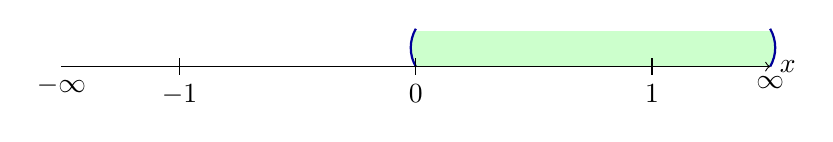
\begin{tikzpicture}[scale=3]
        %colores
        \colorlet{w}{green!20!white}
        \colorlet{bblue}{blue!60!black}

        % Figura relleno
        \fill[w](0,0) arc (210:150:1.5mm) -- +(1.5,0) arc (210:150:-1.5mm) -- cycle;
        % Parentesis, apertura, cierre
        \draw[bblue,thick](0,0) arc (210:150:1.6mm);
        \draw[bblue,thick](1.5,1.6mm) arc (210:150:-1.6mm);

        %Eje y numeracion
        \begin{scope}
            \draw[->] (-1.5,0) -- (1.5,0)node[right] {$x$}coordinate(x axis);
            \draw (-1.5,0) node[below] {$-\infty$}coordinate(x axis);
            \draw (1.5,0) node[below] {$\infty$}coordinate(x axis);
            \foreach \x/\xtext in {-1, 0, 1/-1,0,1}
            \draw[xshift=\x cm] (0pt,1pt) -- (0pt,-1pt) node[below,fill=white] {$\xtext$};
        \end{scope}
    \end{tikzpicture}


\subsection{Sistema de Ecuaciones}

    Un sistema de ecuaciones, es un conjunto de ecuaciones con mas de una
    incógnita, variable, las cuales conforman un problema matemático. Para
    resolverlo se tienen que encontrar los valores de las incógnitas que satisfacen
    las ecuaciones.

    Existen muchos tipos de sistemas de ecuaciones, estos se clasifican según
    que tipo de ecuaciones lo conforman. En este caso se estudiaran los \textbf{
    sistemas de ecuaciones algebraicas}; estos están conformados únicamente por
    ecuaciones algebraicas.

    \textbf{Una ecuación de varias variables} tiene la forma:
    $ a_1X_1+a_2X_2+\cdots+a_nX_n = 0 $ o, también $aX,bY,\cdots,cZ=0$, donde
    $a_1,a_2,\cdots,a_n$ y/o $a,b,z$ son \textbf{coeficientes} y $X_1,X_2,\cdots,X_n$
    y/o $X,Y,\cdots,Z$ son \textbf{variables independientes}.

    Los sistemas tienen la forma general:
    \begin{equation*}
        \left.
        \begin{matrix}
            F_1(x_1,\cdots,x_n)=0\\
            \vdots\\
            F_n(x_1,\cdots,x_n)=0
        \end{matrix}
        \hspace*{0.5cm}\right\rbrace
    \end{equation*}

    Y a su vez, se dividen por sus posibilidades de resolución en:

    \begin{itemize}
        \item \textbf{Compatible determinado}: El sistema siempre tiene solución única.
            Tiene tantas incógnitas como ecuaciones.

        \item \textbf{Compatible indeterminado}: El sistema tiene infinitas soluciones.
            Tiene mas incógnitas que ecuaciones.

        \item \textbf{Incompatible}: El sistema no tiene solución, esto se da por alguna
            incoherencia mientras resolvemos (división por cero, raíz par de un numero
            negativo, incompatibilidad de resultados).
    \end{itemize}

    El sistema compatible indeterminado siempre dependerá de alguna variable,
    quedara expresado en términos de función.

    El compatible determinado siempre dará algún valor \textbf{único} para cada
    variable y es el que se estudiara.

    \subsubsection{Resolución sistemas de ecuaciones}

    Los métodos mas comunes para resolver los sistemas de ecuaciones son:

    \begin{itemize}
        \item sustitución.
        \item igualación.
        \item reducción.
    \end{itemize}

    \textbf{Cabe resaltar que:} existen otros métodos, como lo son el método
    gráfico y los métodos matriciales de Gauss Jordán y kramer.

    \subsubsection*{Sustitución} \label{Sustitucion}

    Consiste en despejar \textbf{una} de las incógnitas, de forma que quede
    $incógnita=expresión$ y luego sustituir en otra ecuación la incógnita
    despejada por la expresión, esto da origen a una
    nueva ecuación la cual tiene una variable menos, repetir hasta que quede
    una ecuación de una sola variable y resolver. Luego se regresan en la linea
    sustituyendo las variables por los nuevos valores resultados.

    Paso a paso se observa:

    \begin{enumerate}
        \item Elegir una ecuación (llámesele ec1) y despejar \textbf{1} incógnita.
        \item Sustituir el despeje en otra ecuación (llámesele ec2), esto
            da origen a una nueva ecuación (llámesele sol).
        \item Verificar si la nueva ecuación (sol) tiene mas de 1 variable.
            \begin{itemize}
                \item Si sol tiene 1 sola variable, se despeja y se obtiene el
                    resultado. Ese resultado se sustituye en ec1 y se obtienen
                    todos los valores
                \item si sol no tiene 1 única variable, despejar alguna otra incógnita
                    y sustituir todos los despejes de incógnitas,
                    en otra ecuación (llámesele ec3) y repetir hasta
                    obtener una única variable.
            \end{itemize}
    \end{enumerate}

Ejemplos:


    \begin{equation*}
        \left.
        \begin{matrix}
            x &+& y &=3\\
            2x &-& y &=0
        \end{matrix}
        \hspace*{0.5cm}\right\rbrace
    \end{equation*}

    Tomando la primera ecuación, procedemos a despejar $x$:

    $$(ec1)\hspace*{1cm} x+y=3 \rightarrow x=3-y $$

    Luego, sustituimos en las segunda ecuación:

    \begin{align*}
        2x-y &= 0		\\
        2(3-y)-y &=0    \\
        2\times3 -2y-y&= 0\\
        6-3y &= 0   \\
        -3y &= -6   \\
        y &= \frac{-6}{-3} \\
        y &= 2\\
    \end{align*}

    y sustituyendo $ Y=2 $ en la $ec1$


    $$ x=3-y \rightarrow x=3-2, \ x=1 $$

    Y el sistema tiene una única solución, dada por los valores:
    $ x=1 $  $ y=2 $.


    Otro ejemplo:

    \begin{equation*}
        \left.
        \begin{matrix}
            \displaystyle\frac{x}{2} &+& 3y &-& z &= 3 \\
            2x &+& 4y &+&5z &= 1\\
            3x &+& 5y &+& 4z &=0
        \end{matrix}
        \hspace*{0.5cm}\right\rbrace
    \end{equation*}

    Despejamos de la primera ecuación $x$:

    \begin{align*}
        (ec1)\hspace*{1cm} \displaystyle\frac{x}{2} +3y-z&=3 \\
        \displaystyle\frac{x}{2} &= 3-3y+z\\
        x&= 2\times(3-3y+z)\\
        x&= 6-6y+2z
    \end{align*}

    Como observamos, hay mas de una variable, por lo tanto, debemos despejar
    una segunda ecuación, y sustituir en una tercera, todos los valores para
    quedar con una sola incógnita:

    De la segunda ecuación, tenemos:

    \begin{align*}
        2x+4y+5z &= 1	\\
        \text{sustituyendo}\\
        2\times(6-6y+2z)+4y+5z &= 1\\
        \text{12 \colorbox{RojoClaro}{-12$y$} \colorbox{AzulClaro}{+4$z$} \colorbox{RojoClaro}{+4$y$} \colorbox{AzulClaro}{+5$z$} }&= \text{1}\\
        -8y + 9z &= -11\\
        \text{Despejamos y} \\
        -8y&= -11-9z \\
        (ec2)\hspace*{1cm} y &= \frac{11+9z}{8}\\
    \end{align*}

    Luego, procedemos a sustituir en la tercera ecuación las expresiones obtenidas
    de $ ec1 $  y $ ec2 $

    \begin{align*}
        3x + 5y + 4z &= 0   \\
        \text{sustituimos, }ec1:\\
        3(6-6y+2z) +5y + 4z &= 0 \\
        \text{18 \colorbox{RojoClaro}{-18$y$} \colorbox{AzulClaro}{+6$z$} \colorbox{RojoClaro}{+5$y$} \colorbox{AzulClaro}{+4$z$}} &= 0\\
        -13y+10z+18&=0\\
        \text{sustituimos, }ec2:\\
        -13\times(\frac{11+9z}{8})+10z &= -18\\
        \frac{-13\times(11+9z)+ 8\times10z}{8}&=-18\\
        -143-117z+80z &=-18\times8\\
        -117z+80z&=-144+143\\
        -37z&=-1\\
        z&=\frac{1}{37}
    \end{align*}

    Regresandonos en las ecuaciones obtenidas, sustituimos
    $\displaystyle z= \frac{1}{37}$  en $ ec2 $:

    \begin{align*}
        y &=\frac{11+9z}{8}  		\\
        y &= \frac{11+9\times\frac{1}{37} }{8}\\
        y &= \frac{11\times37+9}{8\times37} \\
        y&= \frac{52}{37} \\
    \end{align*}

    Finalmente, sustituimos estos valores en $ ec1$:

    \begin{align*}
        x&= 6-6y+2z	\\
        x &= 6- 6\times \frac{52}{37} + 2\times \frac{1}{37}\\
        x&= 6- \frac{312}{37} + \frac{2}{37} \\
        x &= \frac{6\times37 - 312 + 2}{37}\\
        x &=\frac{-88}{37}
    \end{align*}

    y el sistema esta resuelto con:
    \begin{align*}
        x &=\frac{-88}{37} ;& y&=\frac{52}{37} ;& z&=\frac{1}{37}  		\\
    \end{align*}


    \textbf{Como se observa,} este método se volverá mas complicado mientras mayor
    ecuaciones-variables se tengan.

    \subsubsection*{Igualación} \label{Igualacion}

    Este método es muy parecido al de sustitución, consiste en despejar una misma
    variable en las ecuaciones obtenidas e igualarlas (la variable despejada se
    usa como punto común), de esta forma se obtienen
    nuevas ecuaciones las cuales tienen 1 variable menos, se repite el proceso
    hasta tener 1 única ecuación de 1 sola variable, luego se despeja y los valores
    obtenidos se sustituyen en las ecuaciones previamente obtenidas para conseguir
    los resultados.

    Usando los mismos ejemplos que en sustitución:


    \begin{equation*}
        \left.
        \begin{matrix}
            x &+& y &=3\\
            2x &-& y &=0
        \end{matrix}
        \hspace*{0.5cm}\right\rbrace
    \end{equation*}

   procedemos a despejar $x$:

    \begin{align*}
        x+y &=3     & 2x-y&=0 		\\
        x&=3-y      & x&= \frac{y}{2}
    \end{align*}

    Procedemos a igualar en la x:

    \begin{align*}
        3-y &= 	\frac{y}{2} 	\\
        3 &= \frac{y}{2}+y \\
        3 &= \frac{y+2y}{2} \\
        3\times2 &= 3y \\
        y &= \frac{6}{3} \\
        y&=2
    \end{align*}

    luego, sustituimos $y=2$ en cualquiera de las ecuaciones anteriores, usando
    la segunda:

    \begin{align*}
        x&= \frac{y}{2}  		\\
        x&= \frac{2}{2} \\
        x&=1
    \end{align*}

    y el sistema tiene como solución $ x=1 $ y $ y=2 $ (mismo resultado que por
    sustitución ya que la   solución es única).

    Otro ejemplo:

   \begin{equation*}
        \left.
        \begin{matrix}
            \displaystyle\frac{x}{2} &+& 3y &-& z &= 3 \\
            2x &+& 4y &+&5z &= 1\\
            3x &+& 5y &+& 4z &=0
        \end{matrix}
        \hspace*{0.5cm}\right\rbrace
    \end{equation*}

    Despejamos la variable $x$:

    \begin{align*}
        \displaystyle\frac{x}{2} +3y-z &=3   & 2x+4y+5z &= 1             & 3x+5y+4z &= 0 \\
        \displaystyle\frac{x}{2} &= 3-3y+z   & 2x &= 1-4y-5z             & 3x &= -5y-4z  \\
        x&= 2\times(3-3y+z)     & x &= \frac{1-4y-5z}{2}    & x &= \frac{-5y-4z}{3} \\
        x&= 6-6y+2z
    \end{align*}


    Procedemos a igualar las ecuaciones, tenemos que usarlas todas al menos una
    vez, por esto se juntaran la primera con la segunda y la primera con la tercera
    (hay 2 variables restantes así que solo necesitamos 2 ecuaciones):

    \begin{align*}
        6-6y+2z &= \frac{1-4y-5z}{2}    & 6-6y+2z &= \frac{-5y-4z}{3}  		\\
        2\times(6-6y+2z )&= 1-4y-5z     & 3\times(6-6y+2z) &= -5y-4z        \\
        12-12y+4z &= 1-4y-5z            & 18-18y+6z &= -5y -4z \\
        \text{Procedemos a despejar la }y:\\
        -12y+4y &= 1-5z-12-4z           & -18y+5y &= -4z-18-6z \\
        -8y &= -11 -9z                  & -13y    &= -10z -18 \\
        y &= \frac{-11-9z}{-8}          & y &= \frac{-10z-18}{-13} \\
        y&= \frac{11+9z}{8}             & y&= \frac{10z+18}{13}
    \end{align*}

    Ahora que tenemos las 2 ecuaciones despejadas, las volvemos a igualar:

    \begin{align*}
        \frac{11+9z}{8}  &= \frac{10z+18}{13}  		\\
        13\times(11+9z)  &= 8\times(10z+18)     \\
        143+117z &= 80z +144\\
        117z-80z &= 144-143\\
        37z     &= 1 \\
        z &= \frac{1}{37}
    \end{align*}

    Y luego, sustituyendo en alguna ecuación previa, usando la primera ecuación
    despejada de 2 variables  (izquierda):

    \begin{align*}
        y &= \frac{11+9z}{8} \\
        y &= \frac{11+9\times \frac{1}{37} }{8}\\
        y&= \frac{11\times37+9}{37\times8}  \\
        y&= \frac{52}{37} \\
    \end{align*}

    Finalmente, sustituimos estos valores en la primera ecuación:

    \begin{align*}
        x&= 6-6y+2z	\\
        x &= 6- 6\times \frac{52}{37} + 2\times \frac{1}{37}\\
        x&= 6- \frac{312}{37} + \frac{2}{37} \\
        x &= \frac{6\times37 - 312 + 2}{37}\\
        x &=\frac{-88}{37}
    \end{align*}

    y el sistema esta resuelto, dando los mismos valores que por sustitución:
    \begin{align*}
        x &=\frac{-88}{37} ;& y&=\frac{52}{37} ;& z&=\frac{1}{37}  		\\
    \end{align*}


    \subsubsection*{Reducción} \label{Reduccion}

    Este método consiste en reducir la cantidad de ecuaciones-incógnitas que hay
    presente, mediante la suma o resta de las ecuaciones, además de la multiplicación
    o dividiesen de las mismas por un numero entero.

    Para realizar esto, se busca que ambas ecuaciones tengan el mismo coeficiente
    en una determinada variable, luego restarlas si el signo es igual y sumarlas
    si el signo es distinto. de esta forma se obtiene una(s) nueva(s) ecuación(es)
    y se repite el proceso hasta obtener el resultado de una variable, y se
    van sustituyendo los valores progresivamente, como en los métodos anteriores.

    Ejemplos:

    \begin{equation*}
        \left.
        \begin{matrix}
            x &+& y &=3\\
            2x &-& y &=0
        \end{matrix}
        \hspace*{0.5cm}\right\rbrace
    \end{equation*}

    Por facilidad, se procede a ordenar de forma que estén los términos iguales
    uno debajo de otro:

    \begin{equation*}
        \left.
        \begin{matrix}
            x &+& y &=3\\
            2x &-& y &=0
        \end{matrix}
        \hspace*{0.5cm}\right\rbrace
    \end{equation*}

    luego, se multiplica (o divide) una ecuación por un numero el cual de como resultado el
    mismo coeficiente de la otra ecuación en una variable determinada, puede ser
    con el mismo signo(se restaran) o con signos contrarios (se sumaran). Usando
    el signo contrario, se multiplicara la primera ecuación por -2 y se sumara:

    \begin{equation*}
        \left.
        \begin{matrix}
            -2\times(x &+& y &=3)\\
            2x &-& y &=0
        \end{matrix}
        \hspace*{0.5cm}\right\rbrace
    \end{equation*}

    \begin{equation*}
        \begin{matrix}
            -2x &-& 2y &=&-6\\
            2x &-& y &=&0\\
            \hline
            0x &-& 3y &=&-6\\
        \end{matrix}
    \end{equation*}


    $$ y=\frac{-6}{-3} \rightarrow y=2 $$

    Luego, sustituimos en la primera ecuación:
    \begin{align*}
        x+y &=3 \\
        x+2 &=3 \\
        x&=3-2\\
        x&=1
    \end{align*}

    Otro ejemplo:

   \begin{equation*}
        \left.
        \begin{matrix}
            \displaystyle\frac{x}{2} &+& 3y &-& z &= 3 \\
            2x &+& 4y &+&5z &= 1\\
            3x &+& 5y &+& 4z &=0
        \end{matrix}
        \hspace*{0.5cm}\right\rbrace
    \end{equation*}


    En este caso, se toman grupos de 2 ecuaciones. tomando 1 con 2 y 2 con 3:

   \begin{align*}
        \left.
        \begin{matrix}
            \displaystyle\frac{x}{2} &+& 3y &-& z &= 3 \\
            2x &+& 4y &+&5z &= 1\\
        \end{matrix}
        \hspace*{0.5cm}\right\rbrace\hspace*{1cm}&
        \left.
        \begin{matrix}
            2x &+& 4y &+&5z &= 1\\
            3x &+& 5y &+& 4z &=0
        \end{matrix}
        \hspace*{0.5cm}\right\rbrace
    \end{align*}

    Luego, procedemos a multiplicar, para eliminar la variable $x$:

    En el primer conjunto de ecuaciones, la primera ecuación por -4

    En el segundo conjunto de ecuaciones, la primera por -3 y la segunda por 2

    Y sumamos:

   \begin{align*}
        \left.
        \begin{matrix}
           -4\times(\displaystyle\frac{x}{2} &+& 3y &-& z &= 3) \\
            2x &+& 4y &+&5z &= 1\\
        \end{matrix}
        \hspace*{0.5cm}\right\rbrace\hspace*{1cm}&
        \left.
        \begin{matrix}
            -3\times(2x &+& 4y &+&5z &= 1)\\
            2\times(3x &+& 5y &+& 4z &=0)
        \end{matrix}
        \hspace*{0.5cm}\right\rbrace
    \end{align*}




   \begin{align*}
        \begin{matrix}
           -2x &-& 12y &+& 4z &= -12 \\
            2x &+& 4y &+&5z &= 1\\
            \hline
            0x &-& 8y &+&9z &= -11
        \end{matrix}
        \hspace*{1cm}&
        \begin{matrix}
            -6x &-& 12y &-&15z &= -3\\
            6x &+& 10y &+& 8z &=0\\
            \hline
            0x &-&2y &-&-7 &= -3
        \end{matrix}
   \end{align*}

   Luego, se procede a resolver el sistema generado con las dos ecuaciones resultantes:


    \begin{equation*}
        \left.
        \begin{matrix}
           -8y &+&9z &= -11\\
            -2y &-&-7 &= -3
        \end{matrix}
        \hspace*{0.5cm}\right\rbrace
    \end{equation*}

    Multiplicando la segunda ecuación por -4:
    \begin{equation*}
        \left.
        \begin{matrix}
           -8y &+&9z &= -11\\
            -4\times(-2y &-&-7 &= -3)
        \end{matrix}
        \hspace*{0.5cm}\right\rbrace
    \end{equation*}

    \begin{equation*}
        \begin{matrix}
           -8y &+&9z &= -11\\
            8y &+&28 &= 12\\
            \hline
            0y &+&37z &=1
        \end{matrix}
    \end{equation*}


    $$ z = \frac{1}{37}  $$

    luego sustituimos en alguna de las ecuaciones anteriores, sustituyendo en
    la primera:


    \begin{align*}
        -8y &+&9z &= -11\\
        y &= \frac{-11-9z}{8}
        y &= \frac{11+9z}{8} \\
        y &= \frac{11+9\times \frac{1}{37} }{8}\\
        y&= \frac{11\times37+9}{37\times8}  \\
        y&= \frac{52}{37} \\
    \end{align*}

    Finalmente, sustituimos estos valores en la primera ecuación:

    \begin{align*}
        x&= 6-6y+2z	\\
        x &= 6- 6\times \frac{52}{37} + 2\times \frac{1}{37}\\
        x&= 6- \frac{312}{37} + \frac{2}{37} \\
        x &= \frac{6\times37 - 312 + 2}{37}\\
        x &=\frac{-88}{37}
    \end{align*}

    y el sistema esta resuelto, dando los mismos valores que por sustitución o igualación:
    \begin{align*}
        x &=\frac{-88}{37} ;& y&=\frac{52}{37} ;& z&=\frac{1}{37}  		\\
    \end{align*}

